%% Master Thesis Template
%% Please update the specification through this link: https://daim.idi.ntnu.no/howto_thesis_submission.pdf
\documentclass[pdftex,12pt,a4paper,twoside]{book}
\usepackage[lmargin=25mm,rmargin=25mm,tmargin=27mm,bmargin=30mm]{geometry}
\usepackage[utf8]{inputenc}
\usepackage[T1]{fontenc}
\usepackage[english]{babel}

\setlength\parindent{0pt}
\setlength{\parskip}{1em}

\usepackage{setspace}
\usepackage{subcaption}
\usepackage{tikz}
\usepackage{tikz-3dplot}
\usetikzlibrary{shapes, arrows}
\usepackage{pgfplots}
\pgfplotsset{compat=newest}
\usepackage{graphicx}
\graphicspath{{./fig/}{./fig/Intro/}{./fig/Theory/}{./fig/Simulator/}%
{./fig/Implementation/}{./fig/Results/}}
\DeclareGraphicsExtensions{.pdf,.eps,.png,.jpg}

\usepackage{todonotes}

\usepackage{amssymb}
\usepackage{mathrsfs}
\usepackage{amsthm}
\usepackage{amsmath}
\usepackage{color}
\usepackage{array}

\usepackage[symbols,nogroupskip]{glossaries-extra}

\usepackage[pdftex,bookmarks=true]{hyperref}
\usepackage[pdftex]{hyperref}
\hypersetup{
    colorlinks,%
    citecolor=black,%
    filecolor=black,%
    linkcolor=black,%
    urlcolor=black
}

\usepackage{titlesec}
\usepackage{blindtext}
\usepackage{color}
\definecolor{gray75}{gray}{0.75}
\newcommand{\hsp}{\hspace{20pt}}
\titleformat{\chapter}[hang]{\Huge\bfseries}{\thechapter\hsp\textcolor{gray75}{|}\hsp}{0pt}{\Huge\bfseries}

\usepackage[font=small,labelfont=bf]{caption}
\usepackage{fancyhdr}

\usepackage[style=ieee]{biblatex}
\usepackage{csquotes} % to make Biblatex happy
\addbibresource{mylib.bib}

\usepackage{float}
\restylefloat{figure}

\newcommand{\HRule}{\rule{\linewidth}{0.5mm}}

\renewcommand*\contentsname{Table of Contents}

\pagestyle{fancy}
\fancyhf{}
\renewcommand{\chaptermark}[1]{\markboth{\chaptername\ \thechapter.\ #1}{}}
\renewcommand{\sectionmark}[1]{\markright{\thesection\ #1}}
\renewcommand{\headrulewidth}{0.1ex}
\renewcommand{\footrulewidth}{0.1ex}
\fancypagestyle{plain}{\fancyhf{}\fancyfoot[LE,RO]{\thepage}\renewcommand{\headrulewidth}{0ex}}
\makeglossaries

\glsxtrnewsymbol[description={focal length}]{f}{$f$}
\glsxtrnewsymbol[description={Vertical field of view}]{Theta}{$\Theta$}
\glsxtrnewsymbol[description={Horizontal field of view}]{ThetaH}{$\Theta_H$}
\glsxtrnewsymbol[description={Image height in pixels}]{H}{$H$}
\glsxtrnewsymbol[description={Image width in pixels}]{W}{$W$}
\glsxtrnewsymbol[description={Image aspect ratio}]{rho}{$\rho = \frac{H}{W}$}
\glsxtrnewsymbol[description={Point in image world coordinates}]{P}{$\mathbf{P}$}
\glsxtrnewsymbol[description={Point in image plane}]{pi}{$\mathbf{p}$}
\glsxtrnewsymbol[description={Point in quaternion form}]{q}{$\mathbf{q} = [0, \mathbf{p}^\top]^\top$}
\glsxtrnewsymbol[description={Quaternion Rotation from frame i to frame j}]{qji}{$\mathbf{q_{j,i}}$}
\glsxtrnewsymbol[description={Matrix rotation from frame i to frame j}]{Rji}{$\mathbf{R}^j_i$}
\glsxtrnewsymbol[description={Matrix rotation around axis a, by b degrees or radians}]{Rab}{$\mathbf{R}_{a,b}$}
\glsxtrnewsymbol[description={Perspective projection matrix}]{K}{$\mathbf{K}$}
\glsxtrnewsymbol[description={Matrix element on row i and column j}]{Kij}{$\mathbf{K_{ij}}$}
\glsxtrnewsymbol[description={Near end clipping plane}]{dn}{$d_n$}
\glsxtrnewsymbol[description={Far end clipping plane}]{df}{$d_f$}
\glsxtrnewsymbol[description={Longitude}]{theta}{$\theta$}
\glsxtrnewsymbol[description={Latitude}]{phi}{$\phi$}
\glsxtrnewsymbol[description={Sphere radius}]{R}{$R$}
\glsxtrnewsymbol[description={Circle radius}]{r}{$r$}








\begin{document}

%% PART 1
\begin{titlepage}
    \includegraphics[width=0.5\textwidth]{hovedlogo_eng.eps} \hfill\\
    \vspace{2cm} \\
    
    {\Huge{\bfseries 360-degree Camera Simulator for\\Realistic Imaging using Unreal Engine}}
    
    \vspace{2cm}
    
    \Large{\textbf{Sveinung Aanbye Haugane}}
    
    \vfill
    \large{
        \begin{tabbing}
            TTK4550 Specialization Project \\
            Submission date:  \=January 29, 2019 \\
            Supervisor: \>Edmund Førland Brekke, ITK \\
            Co-supervisor: \>Elias Bjørne, ITK \\
        \end{tabbing}
        }
        \vspace{-1cm}
    \large{Norwegian University of Science and Technology, NTNU}\\
    \large{Department of Engineering Cybernetics}
    
\end{titlepage}

%% PART 2
\clearpage
\pagenumbering{roman} 				
\setcounter{page}{1}

\pagestyle{fancy}
\fancyhf{}
\renewcommand{\chaptermark}[1]{\markboth{\chaptername\ \thechapter.\ #1}{}}
\renewcommand{\sectionmark}[1]{\markright{\thesection\ #1}}
\renewcommand{\headrulewidth}{0.1ex}
\renewcommand{\footrulewidth}{0.1ex}
\fancyfoot[LE,RO]{\thepage}
\fancypagestyle{plain}{\fancyhf{}\fancyfoot[LE,RO]{\thepage}\renewcommand{\headrulewidth}{0ex}}

\section*{\Huge Abstract}
\addcontentsline{toc}{chapter}{Abstract}	
$\\[0.5cm]$

While there are many robotics simulators with support for image and video capture, for use in computer vision(CV) applications, few of them are able to capture the complex effects of dynamic shadow and light effects in high-quality graphics environments. Even fewer are able to realistically model the distortion effects applied by wide-angle imaging with a field of view greater than 180 degrees. 

In this project, a simulator for capturing omnidirectional fisheye lens distorted images is presented, with the ability to capture pictures with a 270-degree vertical field of view, utilizing Unreal Engine's graphical software as a basis to create and simulate the scenery. The fisheye camera module is built as a client program to the open source AirSim simulator, developed by Microsoft. Taking advantage of their already existing perspective image capture module and multirotor vehicle, five 90-degree field of view cameras are set up underneath, providing a constant stream of perspective images. These images are then mapped to a single fisheye-distorted image, with the added possibility to distribute it over a Robot Operating System(ROS) network. This opens up the possibilities to test computer vision navigation algorithms on realistic images, with realistic light effects, making it easier to develop methods that are robust to difficult lighting conditions. As the fisheye camera uses the versatile format of the OpenCV image matrix, this module can also be transferred into other OpenCV projects, with only small changes to the code. 



\clearpage
\section*{\Huge Preface}
\addcontentsline{toc}{chapter}{Preface}
$\\[0.5cm]$

The presented work in this report is result of the 9th term project of the Master of Science program in the field of Cybernetics and Robotics, at the Norwegian University of Science and Technology, NTNU. The project counts as 15, out of the semester total of 30 credit points. This means that there is substantial amounts of work behind it.

I would like to thank my supervisors Edmund F. Brekke and Elias S. Bjørne for the guidance and support along the way. Especially Mr. Bjørne, who has set aside a significant amount of his time to help read through, discuss and steer this project report in the right direction.


\cleardoublepage


\addcontentsline{toc}{chapter}{Table of Contents}
\tableofcontents
\clearpage
\printunsrtglossary[type=symbols,style=long,title={List of Symbols}]
\clearpage

\section*{{\Huge Abbreviations}}
\addcontentsline{toc}{chapter}{Abbreviations}
$\\[0.5cm]$

\noindent 
\begin{center}
\begin{tabular}{ l c l }
    API & = & Application Program Interface \\
    CCD & = & Charge-Coupled Device \\
    CGI & = & Computer-Generated Imagery \\
    CUDA & = & Compute Unified Device Architecture \\
    CV & = & Computer Vision \\
    FoV & = & Field of View \\
    GNSS & = & Global Navigation Satellite System \\
    GPS & = & Global Positioning System \\
    GPU & = & Graphics Processing Unit \\
    HITL & = & Hardware in the Loop \\
    HNMSIM & = & Hybrid Networked Multi-agent Simulator \\
    IMU & = & Inertial Measurement Unit \\
    IP & = & Internet Protocol \\
    ISO & = & Standardised exposure index for cameras \\
    LIDAR & = & Light Imaging, Detection And Ranging \\
    Mac & = & Macintosh \\
    MAV & = & Micro Aerial Vehicle \\
    NASA & = & National Aeronautics and Space Administration \\
    NTNU & = & Norwegian University of Science and Technology \\
    OpenCV & = & Open Source Computer Vision Library \\
    OpenCL & = & Open Computing Language \\
    OS & = & Operating System \\
    PC & = & Personal Computer \\
    PNG & = & Portable Network Graphics \\
    RBGA & = & Red, Green, Blue, Alpha \\
    ROS & = & Robot Operating System \\
    RPC & = & Remote Procedure Call \\
    SLAM & = & Simultaneous Localization and Mapping \\
    SVO & = & Semi-direct Visual Odometry \\
    TCP & = & Transfer Control Protocol \\
    UAV & = & Unmanned Aerial Vehicle \\
    VIO & = & Visual Inertial Odometry \\
    VO & = & Visual Odometry \\
    V-REP & = & Virtual Robot Experimentation Platform \\
    VSLAM & = & Visual Simulataneous Localization and Mapping \\
    XML & = & Extensible Markup Language \\
\end{tabular}
\end{center}

\cleardoublepage

\pagestyle{fancy}
\fancyhf{}
\renewcommand{\chaptermark}[1]{\markboth{\chaptername\ \thechapter.\ #1}{}}
\renewcommand{\sectionmark}[1]{\markright{\thesection\ #1}}
\renewcommand{\headrulewidth}{0.1ex}
\renewcommand{\footrulewidth}{0.1ex}
\fancyfoot[LE,RO]{\thepage}
\fancyhead[LE]{\leftmark}
\fancyhead[RO]{\rightmark}
\fancypagestyle{plain}{\fancyhf{}\fancyfoot[LE,RO]{\thepage}\renewcommand{\headrulewidth}{0ex}}

\pagenumbering{arabic} 				
\setcounter{page}{1}
%% PART 3 -- The Chapters
\pagenumbering{arabic} 				
\setcounter{page}{1}
%===================================== CHAP 1 =================================

\chapter{Introduction}

This will be the introduction. Reference to symbol: $\gls{p}$. Reference to Airsim paper: \cite{Airsim_paper}


\section{Previous work}

\todo[inline]{Should contain work related to 360 cameras, modeling of 360 degree projections and what approaches there has been to simulating 360 footage}

\chapter{Background and theory}
\section{Modeling of cameras}

All cameras project a 3D scene onto a 2D plane. This causes information to be lost about the depth of the image. It is therefore not possible to calculate the exact placement of an object from a single picture unless there is extra information about the objects in the picture. For this reason, it is easy to create a projection of a 3D scene, but hard to create a scene from a projection. In addition to this, the number of pixels and the field of view(FoV) also affect the information and detail in the captured image. The most basic camera model is called the pinhole model, and it is applicable for most cameras without high distortion lenses.

\subsection{Pinhole projection} \label{sec:pinhole}
The pinhole model is based on the Camera Obscura, made in 1568. It captures a scene by projecting straight light rays through a common focal point, and through a plane. The projection itself is made from where the light rays intersect the projection plane. The focal length, $f$, and the image plane size will decide the FoV, $\Theta_H$ and $\Theta$, as shown in Figure~\ref{fig:pinhole}. 

\begin{figure}[!htb]
    \centering

    \tdplotsetmaincoords{80}{145}
    \begin{tikzpicture}[tdplot_main_coords, scale = 1.8]
    
        \tdplotsetrotatedcoords{0}{-90}{90}
        \draw[tdplot_rotated_coords, ->] (-0.7,0,0) -- (2,0,0) node[below right]{$X$};
        \draw[tdplot_rotated_coords, ->] (0,-0.5,0) -- (0,1,0) node[right]{$Y$};
        \draw[tdplot_rotated_coords, dashed, opacity=0.7] (0,0,-0.5) -- (0,0,9.2);
        \draw[tdplot_rotated_coords, ->] (0,0,9.2) -- (0,0,10) node[below]{$z,Z$};
        
        \pgfmathsetmacro{\rvec}{8}
        \pgfmathsetmacro{\imgradius}{3}
        \pgfmathsetmacro{\thetavec}{12}
        \pgfmathsetmacro{\phivec}{8}
        
        \coordinate (O) at (0,0,0);
        \tdplotsetcoord{P1}{\rvec}{90 -\phivec}{180 - \thetavec}
        \tdplotsetcoord{longP1}{\rvec*1.1}{90 -\phivec}{180 - \thetavec}
        \tdplotsetcoord{P2}{\rvec}{90 +\phivec}{180 - \thetavec}
        \tdplotsetcoord{longP2}{\rvec*1.1}{90 +\phivec}{180 - \thetavec}
        \tdplotsetcoord{P3}{\rvec}{90 + \phivec}{180 + \thetavec}
        \tdplotsetcoord{longP3}{\rvec*1.1}{90 +\phivec}{180 + \thetavec}
        \tdplotsetcoord{P4}{\rvec}{90 - \phivec}{180 + \thetavec}
        \tdplotsetcoord{longP4}{\rvec*1.1}{90 -\phivec}{180 + \thetavec}
        
        \tdplotsetcoord{IMG1}{\imgradius}{90 -\phivec}{180 - \thetavec}
        \tdplotsetcoord{IMG2}{\imgradius}{90 +\phivec}{180 - \thetavec}
        \tdplotsetcoord{IMG3}{\imgradius}{90 +\phivec}{180 + \thetavec}
        \tdplotsetcoord{IMG4}{\imgradius}{90 -\phivec}{180 + \thetavec}
        \coordinate (IMGC) at (-2.906,0,0);
        
        \shade[tdplot_rotated_coords, ball color=blue!50, opacity = 0.9] (0,0,8) circle (1cm); 

        \tdplotsetrotatedcoordsorigin{(IMGC)} %\imgradius*sin(90-\phivec)*cos(180-\thetavec)
        \shade[tdplot_rotated_coords, ball color=blue!50, opacity = 0.9] (0,0,0) circle (0.375);
        \draw[tdplot_rotated_coords, ->] (-0.7,0,0) -- (2,0,0) node[below right]{$x$};
        \draw[tdplot_rotated_coords, ->] (0,-0.5,0) -- (0,1,0) node[right]{$y$};
        
        \draw[] (IMG1) -- (IMG2) -- (IMG3) -- (IMG4) -- cycle;
      
        \draw[] (0,0,0.75) -- (0,0,0.85); \draw[] (0,0,0.8) -- (-2.906,0,0.8); \draw[] (-2.906,0,0.75) -- (-2.906,0,0.85);
        \draw[] (-1.45,0,1) node{$f$};
        
        \draw[thick, opacity = 0.3] (O) -- (P1); \draw[dashed, opacity = 0.3] (P1) -- (longP1);
        \draw[thick, opacity = 0.3] (O) -- (P2); \draw[dashed, opacity = 0.3] (P2) -- (longP2);
        \draw[thick, opacity = 0.3] (O) -- (P3); \draw[dashed, opacity = 0.3] (P3) -- (longP3);
        \draw[thick, opacity = 0.3] (O) -- (P4); \draw[dashed, opacity = 0.3] (P4) -- (longP4);
        
        \tdplotsetthetaplanecoords{180-\thetavec}
        \tdplotdrawarc[tdplot_rotated_coords]{(O)}{5}{90-\phivec}{90+\phivec}{anchor=west}{$\Theta$}
        \tdplotsetrotatedcoords{0}{\phivec}{90}
        \tdplotdrawarc[tdplot_rotated_coords]{(O)}{5}{90-\thetavec}{90+\thetavec}{anchor=south}{$\Theta_H$}
        
        
    \end{tikzpicture}

    \caption{Pinhole projection with the image plane between the focal point and the object.}
    \label{fig:pinhole}
    
\end{figure}

Using the properties of similar triangles, the relationship between the world coordinates, $X,Y,Z$, and the image coordinates $x,y$ becomes:

\begin{align}
    tan(\phi_x) &= \frac{x}{f} = \frac{X}{Z} & tan(\phi_y) &= \frac{y}{f} = \frac{Y}{Z} \label{eq:pinhole_tan_relation} \\
    x &= f\frac{X}{Z} & y &=f\frac{Y}{Z}
    \label{eq:pinhole_relation}
\end{align}

As seen in Equation \eqref{eq:pinhole_relation}, the relationship between the sizes are nonlinear. In order to present this in matrix form, the homogenous coordinates, $\mathbf{p}^c=[x,y,1]^\top$, and $\mathbf{P}^c=[X,Y,Z,1]^\top$ are used. The matrix transformation is shown in Equation~\eqref{eq:pinhole_matrix}, with the intermediate step $\mathbf{\Tilde{p}}^c$ being $\mathbf{p}^c$ scaled by $Z$. The $\bullet^c$ superscript refers to the camera coordinate frame.

\begin{align}
    \mathbf{\Tilde{p}}^c &= \begin{bmatrix}
        \Tilde{x} \\ \Tilde{y} \\ \Tilde{z}
    \end{bmatrix} = \begin{bmatrix}
        f & 0 & 0 & 0 \\
        0 & f & 0 & 0 \\
        0 & 0 & 1 & 0
    \end{bmatrix}\begin{bmatrix}
        X \\ Y \\ Z \\ 1
    \end{bmatrix} &
    \mathbf{p}^c &= \frac{1}{\Tilde{z}}\mathbf{\Tilde{p}}^c
    \label{eq:pinhole_matrix}
\end{align}

Since the light rays need to pass through the pinhole and onto the image plane, it is not possible to have a FoV larger than $180^\circ$. As seen in Equation~\eqref{eq:pinhole_matrix}, the projected object is also scaled by the distance, causing the points where the vertical FoV is $180^\circ$ to be singular. 

\begin{figure}[!htb]
    \centering
    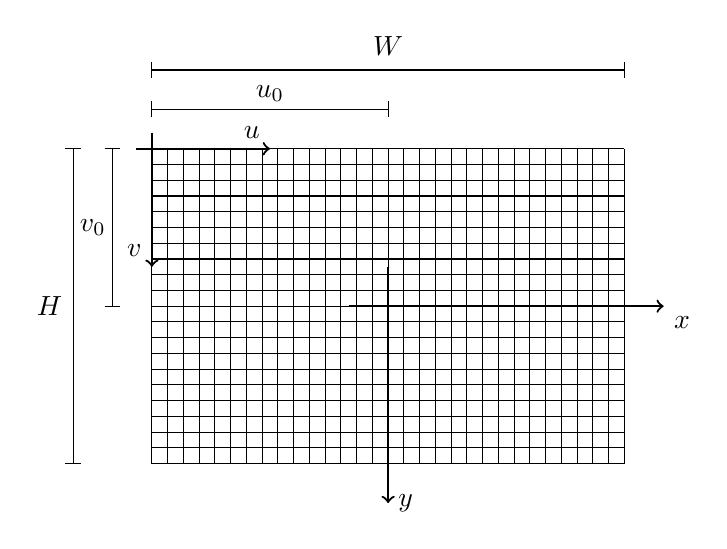
\begin{tikzpicture}[scale = 1.0]
    
    \draw[thick, ->] (-0.5,0,0) -- (3.5,0,0) node[below right]{$x$};
    \draw[thick, ->] (0,0.5,0) -- (0,-2.5,0) node[right]{$y$};
    \draw[thick, ->] (-3.2,2,0) -- (-1.5,2,0) node[above left]{$u$};
    \draw[thick, ->] (-3,2.2,0) -- (-3,0.5,0) node[above left]{$v$};
    
    \draw[] (-3,3,0) -- (3,3,0); \draw[] (-3,2.9,0) -- (-3,3.1,0); \draw[] (3,2.9,0) -- (3,3.1,0);
    \draw[] (-3,2.5,0) -- (0,2.5,0); \draw[] (-3,2.4,0) -- (-3,2.6,0); \draw[] (0,2.4,0) -- (0,2.6,0);
    \draw[] (-1.5,2.7,0) node{$u_0$};
    \draw[] (0,3.3,0) node{$W$};
    
    \draw[] (-4,2,0) -- (-4,-2,0); \draw[] (-4.1,2,0) -- (-3.9,2,0); \draw[] (-4.1,-2,0) -- (-3.9,-2,0);
    \draw[] (-3.5,2,0) -- (-3.5,0,0); \draw[] (-3.6,2,0) -- (-3.4,2,0); \draw[] (-3.6,0,0) -- (-3.4,0,0);
    \draw[] (-3.75,1,0) node{$v_0$};
    \draw[] (-4.3,0,0) node{$H$};
    
    \foreach \yline in {-2,-1.8,...,2} {
        \draw[] (-3, \yline, 0) -- (3, \yline, 0);
    } %end foreach
    
    \foreach \xline in {-3,-2.8,...,3} {
        \draw[] (\xline, -2, 0) -- (\xline, 2, 0);
    } %end foreach
    
    \end{tikzpicture}
    
    \caption{Relationship between pixel and image coordinates.}
    \label{fig:rel_img_pixel}
\end{figure}

In a digital camera, the image plane consists of a small chip with a discrete amount of light sensitive elements, or pixels. A new pixel coordinate frame is defined to consist of the image pixels, with the origin in the upper left corner, as shown in Figure~\ref{fig:rel_img_pixel}. Using $W$ and $H$ as the image width and height in pixels, respectively, the transformation from image coordinates to pixel coordinates will be as shown in Equation~\eqref{eq:pixel_transform}, with $\bullet^p$ referring to the pixel coordinate frame, with its origin at the camera center.

\begin{equation}
    \mathbf{p}^p = \begin{bmatrix}
        u \\ v \\ 1
    \end{bmatrix} = \begin{bmatrix}
        \frac{W}{2x_{max}} & 0 & u_0 \\
        0 & \frac{H}{2y_{max}} & v_0 \\
        0 & 0 & 1
    \end{bmatrix} \mathbf{p}^c =
    \begin{bmatrix}
        \frac{W}{2x_{max}} & 0 & \frac{W}{2} \\
        0 & \frac{H}{2y_{max}} & \frac{H}{2} \\
        0 & 0 & 1
    \end{bmatrix}\begin{bmatrix}
        x \\ y \\ 1
    \end{bmatrix}
    \label{eq:pixel_transform}
\end{equation}

\section{Distortions and wide angle pictures}

Wide angle image capture usually refers to pictures taken with a FoV greater than $60^\circ$. Increasing the field of view lets the camera capture more of the scene. However, the details also have to be compressed in order to fit in the image. This creates a trade-off between the amount of the scene captured and the level of detail. Increasing the resolution will reduce the amount of detail lost, but doing so also increases the amount of computation time needed to process the images.

As described in Section~\ref{sec:pinhole}, pinhole cameras are not able to capture elements that are straight to the side or behind the camera. This singularity can also be seen in Figure~\ref{fig:wide_angle_pinhole_nolens}, where the image plane would need to be infinitely large to capture elements at $90^\circ$ to either side. In order to reliably capture wide angle pictures, wide-angle cameras take advantage of lens distortion. Figure~\ref{fig:wide_angle_pinhole_lens} shows how a lens may be utilized to capture a wide-angle picture onto a smaller image plane. The downside of this method is that elements towards the edges of the picture become compressed, causing straight lines to appear curved in the image. This type of distortion is called barrel distortion. Lenses that create barrel distortion in all radial directions from the image center is called a fisheye lens, and are used in many wide angle cameras.

\begin{figure}[!htb]
    \centering
    \begin{subfigure}[b]{0.45\textwidth}
    \centering
    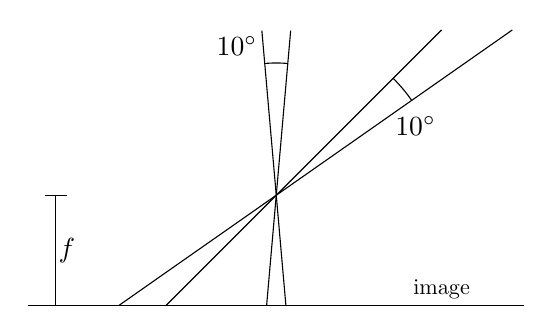
\begin{tikzpicture}[scale=0.7]
        \pgfmathsetmacro{\rvecimg}{2}
        \pgfmathsetmacro{\rvecscene}{3}
        
        \draw[] (0,0,0) -- (95:\rvecscene); \draw[] (0,0,0) -- (85:\rvecscene); 
        \draw[] (0,0,0) -- (-95:\rvecimg); \draw[] (0,0,0) -- (-85:\rvecimg);
        \draw[] (95:0.8*\rvecscene) arc (95:85:0.8*\rvecscene); \draw[] (90:0.9*\rvecscene) node[xshift=-0.5cm]{$10^\circ$};
        
        \draw[] (0,0,0) -- (45:1.414*\rvecscene); \draw[] (0,0,0) -- (35:1.743*\rvecscene); 
        \draw[] (0,0,0) -- (-135:1.414*\rvecimg); \draw[] (0,0,0) -- (-145:1.743*\rvecimg);
        \draw[] (45:\rvecscene) arc (45:35:\rvecscene); \draw[] (40:1.1*\rvecscene) node[yshift=-0.6cm]{$10^\circ$};
        
        \draw[] (-4.5,-\rvecimg,0) -- (4.5,-\rvecimg,0);
        \draw[] (3,-\rvecimg + 0.3,0) node[scale=0.8]{image};
        
        \draw[] (-4,-\rvecimg,0) -- (-4,0,0);
        \draw[] (-4.2,0,0) -- (-3.8,0,0);
        \draw[] (-3.8, -0.5*\rvecimg,0) node{$f$};
        
    \end{tikzpicture}
    \caption{Without lens distortion.}
    \label{fig:wide_angle_pinhole_nolens}
    \end{subfigure}
    \begin{subfigure}[b]{0.45\textwidth}
    \centering
    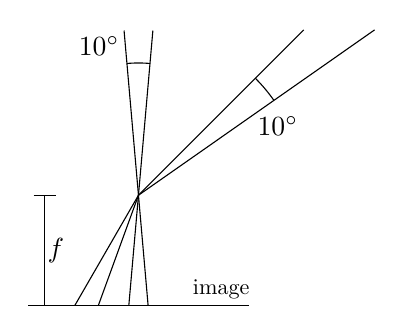
\begin{tikzpicture}[scale=0.7]
        \pgfmathsetmacro{\rvecimg}{2}
        \pgfmathsetmacro{\rvecscene}{3}
        
        \draw[] (0,0,0) -- (95:\rvecscene); \draw[] (0,0,0) -- (85:\rvecscene); 
        \draw[] (0,0,0) -- (-95:\rvecimg); \draw[] (0,0,0) -- (-85:\rvecimg);
        \draw[] (95:0.8*\rvecscene) arc (95:85:0.8*\rvecscene); \draw[] (90:0.9*\rvecscene) node[xshift=-0.5cm]{$10^\circ$};
        
        \draw[] (0,0,0) -- (45:1.414*\rvecscene); \draw[] (0,0,0) -- (35:1.743*\rvecscene); 
        \draw[] (0,0,0) -- (-110:1.064*\rvecimg); \draw[] (0,0,0) -- (-120:1.155*\rvecimg);
        \draw[] (45:\rvecscene) arc (45:35:\rvecscene); \draw[] (40:1.1*\rvecscene) node[yshift=-0.6cm]{$10^\circ$};
        
        \draw[] (-2,-\rvecimg,0) -- (2,-\rvecimg,0);
        \draw[] (1.5,-\rvecimg + 0.3,0) node[scale=0.8]{image};
        
        \draw[] (-1.7,-\rvecimg,0) -- (-1.7,0,0);
        \draw[] (-1.9,0,0) -- (-1.5,0,0);
        \draw[] (-1.5, -0.5*\rvecimg,0) node{$f$};
        
    \end{tikzpicture}
    \caption{With lens distortion.}
    \label{fig:wide_angle_pinhole_lens}
    \end{subfigure}
    
    \caption{Amount of image space for different parts of the scene, using a pinhole camera, with and without a camera lens.}
    \label{fig:wide_angle_pinhole}
    
\end{figure}

\subsection{Fisheye projection}

The lens distortion of a fisheye lens can be visualized and modeled through projecting the scene onto a sphere and then project that sphere onto an image plane. Using spherical coordinates makes it is easier to describe points in the image plane, as the radial distance on the image plane is directly coupled to the angle a feature makes with the z-axis. Figure~\ref{fig:fisheye_spherical_projection} visualizes the projection, where the red lines represent a constant angle $\phi$.

Using the relationship between spherical and cartesian coordinates, $X = Rsin(\phi)cos(\theta)$, $Y = Rsin(\phi)sin(\theta)$ and $Z = Rcos(\phi)$, the polar coordinates $[R,\theta,\phi]^\top$ become:

\begin{equation}
    \begin{aligned}
        R = X^2 &+ Y^2 + Z^2 \\
        \theta = atan2\left(Y,X\right)\quad  ,& \quad \phi = atan2\left(\sqrt{X^2 + Y^2},Z\right)
    \end{aligned}
    \label{eq:theory_polar_coords}
\end{equation}

\begin{figure}[!htb]
    \centering
    \tdplotsetmaincoords{70}{160}
    \begin{tikzpicture}[tdplot_main_coords, scale = 1.4]
    
    \coordinate (O) at (0,0,0);
    \tdplotsetrotatedcoords{0}{-90}{90}
    \draw[tdplot_rotated_coords, ->] (-0.5,0,0) -- (6,0,0) node[below right]{$X$};
    \draw[tdplot_rotated_coords, ->] (0,-0.5,0) -- (0,2.5,0) node[right]{$Y$};
    \draw[tdplot_rotated_coords, dashed] (0,0,-2.5) -- (0,0,6);
    \draw[tdplot_rotated_coords, ->] (0,0,6) -- (0,0,8) node[below]{$z,Z$};
    
    \tdplotsetcoord{P}{6}{65}{150}
    \draw[] (P) node[above right]{$\mathbf{P}^c$}; \node at (P){\textbullet};
    \draw[] (O) -- (P);
    
    \tdplotsetcoord{ROTORIG}{7}{90}{180}
    \tdplotsetrotatedcoordsorigin{(ROTORIG)}
    \draw[tdplot_rotated_coords, ->] (180:0.3) arc (180:360:0.3);
    \draw[tdplot_rotated_coords] (0,-0.5,0) node{$\theta$};
    
    \tdplotsetcoord{IMGC}{2}{90}{0}
    \tdplotsetrotatedcoordsorigin{(IMGC)}
    \foreach \x in {-2,-1.5,...,2} {
        \draw[tdplot_rotated_coords] (\x,-2) -- (\x,2);
    }
    \foreach \y in {-2,-1.5,...,2} {
        \draw[tdplot_rotated_coords] (-2,\y) -- (2,\y);
    }
    \foreach \phi in {10,20,...,80} {
        \draw[tdplot_rotated_coords, color=red, opacity = 0.8] (0,0) circle({\phi/45});
    }
    \draw[tdplot_rotated_coords, thick, opacity = 0.8] (0,0) circle(2);
    
    \draw[tdplot_rotated_coords, ->] (-0.5,0,0) -- (4,0,0) node[below right]{$x$};
    \draw[tdplot_rotated_coords, ->] (0,-0.5,0) -- (0,2.5,0) node[right]{$y$};
    \draw[tdplot_rotated_coords, ->] (-2.5,-2,0) -- (2,-2,0) node[below right]{$u$};
    \draw[tdplot_rotated_coords, ->] (-2,-2.2,0) -- (-2,2,0) node[below]{$v$};
    
    \draw[tdplot_rotated_coords] (0,-2.3,0) -- (0,-2.3,2);
    \draw[tdplot_rotated_coords] (0,-2.2,0) -- (0,-2.4,0); \draw[tdplot_rotated_coords] (0,-2.2,2) -- (0,-2.4,2);
    \draw[tdplot_rotated_coords] (0,-2.5,1) node{$f$};
    
    \tdplotsetrotatedcoordsorigin{(O)}
    \draw[thick, tdplot_rotated_coords] (0:2) arc (0:360:2); 
    \foreach \angle in {-90,-95,...,-270} {
        \tdplotsetrotatedcoords{90}{\angle}{0}
        \draw[tdplot_rotated_coords, opacity = 0.7] (0:2) arc (0:180:2);
        
    }
    
    \foreach \angle in {10,20,...,80} {
        \coordinate (TMP) at ({-2*cos(\angle)},0,0);
        \tdplotsetrotatedcoordsorigin{(TMP)}
        \draw[tdplot_rotated_coords, color = red] (0:{2*sin(\angle)}) arc (0:360:{2*sin(\angle)});
    }
    
    \tdplotsetrotatedcoords{90}{-43}{0}
    \draw[tdplot_rotated_coords, ->] (90:5) arc (90:52:5);
    \draw[tdplot_rotated_coords] (70:5.3) node{$\phi$};
    
    \end{tikzpicture}
    
    \caption{Equiangular fisheye lens projection. Focal length exaggerated for visual purposes.}
    \label{fig:fisheye_spherical_projection}
\end{figure}

In order to project the unit sphere onto a plane, different models exist. All of these describe lens types, providing different distortions models for the fisheye camera. Table~\ref{tab:theory_fisheye_lens_model} shows four different lens models used for fisheye cameras. The $r(\phi)$ represents the distance from the image center in the fisheye image plane. the relationship between the polar image coordinates $[r(\phi), \theta]^\top$ and the image coordinates $[x,y]^\top$ in Figure~\ref{fig:fisheye_spherical_projection}, can be seen in Equation~\eqref{eq:theory_equiangular_coords}. The mapping to pixel coordinates $[u,v]^\top$ is the same as described in Equation~\eqref{eq:pixel_transform}, where $x_{max}$ and $y_{max}$ is decided by $||r(\phi)||_2$.

\begin{align}
    r(\phi) &= f \cdot \phi & \theta &= \theta \nonumber \\
    x &= rcos(\theta) & y &= rsin(\theta)
    \label{eq:theory_equiangular_coords}
\end{align}

The equiangular used in the above example is the simplest and only incorporates radial distortion. In \cite{FisheyeCorke}, the models shown in Table~\ref{tab:theory_fisheye_lens_model} are presented. Another type of model is shown in Matlab's calibration guide for fisheye lens cameras\cite{MatlabFish}. This guide uses a model presented in \cite{FisheyeKalibration}, in addition to the ability to apply a stretch matrix and set distortion center. This model therefore provides much more customizability.

\begin{table}[!htb]
    \centering
    \caption{Four different lens models for fisheye projection.}
    \label{tab:theory_fisheye_lens_model}
    \begin{tabular}{|c|c|} \hline
        Lens model & radius $r(\phi)$ \\ \hline
        Equiangular & $k_1\phi$\\ \hline
        Stereographic & $k_1 tan\left(\frac{\phi}{2}\right)$\\ \hline
        Equisolid & $k_1 sin\left(\frac{\phi}{2}\right)$\\ \hline 
        Polynomial & $k_1 \phi + k_2 \phi^2 + ...$\\ \hline
    \end{tabular}
\end{table}

\subsection{Cylindrical projection}

The goal of the cylindrical projection and camera types is to reduce the radial distortion and feature compression while maintaining the ability to capture images with a horizontal FoV larger than $180^o$. Along the vertical y-axis, the cylindrical projection functions like a pinhole projection, where the mapping is identical to Equation~\eqref{eq:pinhole_relation}. For the horizontal axis, the polar coordinate $\theta$ is used, such that the mapping to the image plane becomes:

\begin{subequations}
\begin{equation}
    \theta = atan2\left(X,Z\right)
    \label{eq:cylindrical_theta}
\end{equation}
\begin{equation}
    y = R\frac{Y}{Z}
    \label{eq:cylindrical_y}
\end{equation}
\label{eq:cylindrical}
\end{subequations}

Theoretically this representation removes all vertical radial distortion. However, it is still subject to the introduction of distortion through imperfect lenses or image plane alignment. Using the same vertical mapping as the pinhole model also limits the vertical FoV in the same manner as it would for the pinhole camera. Cameras using this projection types are not that common. However, this projection type is highly suited to project and stitch pictures taken by a camera rotating around an axis, and is frequently used in panorama capture modes on digital cameras or mobile phones.

\subsection{Catadioptric projection}

Using internal mirrors to reflect the light, catadioptric lenses can achieve large focal lengths without increasing the physical length of the objective. This makes the technology ideal for telescopes and narrow-angle imaging. The same principle has been developed to include large FoV cameras and panoramic imaging, as seen in \cite{CatadioptricOmni}. 

\begin{figure}[!htb]
    \centering
    \includegraphics[width=0.6\textwidth]{rapport/fig/Theory/cata.jpeg}
    \caption{A simple catadiotric lens showing the central mirror, producing the blind spot \cite{CataImage}.}
    \label{fig:theory_catadioptric_lens}
\end{figure}

Figure~\ref{fig:theory_catadioptric_lens} shows a simplified catadioptric mirror setup. Here it can be seen that the mirror has to be placed within the FoV. This means that the catadioptric lens will always cause a blind spot. Shadows of the mirror mount may also appear in the image. To reduce this effect, the mount has to be made quite fragile. This makes the cameras unsuited for applications with significant vibrations.

The pixel mapping and FoV are highly dependent on the reflective surface used. Most surfaces will introduce similar radial distortions to the fisheye lens, but there has been developed catadioptric lenses producing rectilinear projections \cite{RectilinearCatadioptric}. However, this has to be mounted at a fixed distance from the ground, making them unfit for moving objects. Nayar S. K. made a wide angle catadioptric lens \cite{CatadioptricOmni} with a single viewpoint and proposes further a setup where two of these are mounted back to back to produce a full spherical image.

\subsection{Panomorph projection}

The panomorph lens types are designed around a non-uniform distribution of pixels within the FoV and is patented by ImmerVision. This creates an opportunity to focus on important parts of the FoV, and enhance the resolution in these parts. This can counteract the problems that wide-angle cameras have with the reduced angular resolution, without increasing the image resolution. The non-uniform pixel distribution can also be tweaked to use more of the image sensors area \cite{PanomorphLowCostSurvailance}, and therefore utilize more of the available resolution.

Different types of panomorph lenses have been proposed for different applications. In 2010 it was proposed to use a panomorph lens in endoscopy\cite{endoscopypano}. This lens is based on the human eye, and has increased resolution around the center of vision. Other applications include security cameras\cite{PanomorphEnhancesSurvailance}, where the outlying areas have been given an increased resolution, to counteract the compact representation provided by normal fisheye cameras.

The panomorph lens is both harder to construct and model, due to its uneven pixel distribution within the FoV. As it closely resembles the fisheye lens, one could possibly achieve a quite good calibration using the polynomial model in \ref{tab:theory_fisheye_lens_model}, or the unified model presented in \cite{FisheyeKalibration}, as they both support nonlinear radial distortion. The polynomial model would need to be augmented with stretch parameters, however.

\section{Computer graphics}

Our eyes, and cameras, capture the 3D world from light hitting photosensitive elements. This means that an object directly or partly behind another object will be hidden in the picture unless it is captured by a reflection. In addition to this, shadows, colors, and lighting of objects in the scene are all based on how the light rays bounce around in the room, and how they eventually hit the camera lens. In computer graphics, there is no inherent concept of light. This means that all the effects that are based around light must be estimated or simulated. Since calculating light and shadow effects are quite expensive computationally, it is not uncommon to add shadow elements directly to the object texture, in order to optimize for speed.

There are two main approaches to simulating light. One approach is Ray tracing, which traces light-rays as they travel in straight lines from the camera center. When a ray hits an object, the ray is split in two, creating a shadow ray following the same trajectory through the object, and a reflection ray following the reflection trajectory. Ultimately these rays will either find a light source or leave the scene. Usually, the rays are limited to a specific number of bounces to save some computation time. This technique is incredibly powerful and is used heavily in Computer Graphics Imagery(CGI) for film making. However, the amount of computation necessary makes it hard to incorporate this in real-time applications.

The other approach is often referred to as rasterization, and it is the one used the most in real-time applications. Rasterization is a step in a larger pipeline of graphics computations, choosing which element to draw to which pixel. The main advantage of rasterization is its short computation time and ability to be parallelized, as processing speed is very important in real-time graphics production. The efficiency of rasterization has also driven the graphics cards to be as effective as they are today. The downside of rasterization is that it loses a lot of information about the lighting in the scene, providing the shader with much less information for the final coloring.

\subsection{Graphics projection}

Before the rasterization and the coloring(shading) of the pixels can be done, the visibility problems must be solved. This is one of the main difficulties in graphics programming. In simple terms, this consists of two tasks: \emph{Clipping}, which is the process of removing the parts that are outside the FoV, and \emph{culling}, the process of deciding what is visible to the camera. While clipping of the FoV is straight forward, culling is not. The problem comes with transparency and reflections, where objects that are behind others, should still be visible or contribute to the final pixel color. 

In order to do these tasks efficiently, and to be able to use the same algorithms on different projection types, the scene is first projected into a normalized volume. This means that a projection in computer graphics is referencing a volume transformation in $\mathbb{R}^3$, instead of a transformation from $\mathbb{R}^3 \rightarrow \mathbb{R}^2$, which is the case for camera projections. The final transformation to an image plane happens in the rasterization and shading algorithm.

There are two main projection types used: \emph{orthographic} and \emph{perspective}. Orthographic projection is specially made to keep the scale of the object independent on how far away it is from the camera. This makes it ideal for schematics and other computer-aided design(CAD), where the size of the drawing must be proportional to the real size of the object. The other type is perspective projection, and it will be the one that is relevant for this project.

\subsection{Perspective projection}

The goal of perspective projection is to compress the scene into a normalized volume, while still conserving the perspective properties. This means that object sizes are scaled with distance, the same way as in a pinhole camera. In Figure~\ref{fig:perspective_proj_yz}, a side view of this process is shown, in the yz-plane. The image shows two points, $a$ and $b$, as well as their projected counterparts, $a^*$ and $b^*$, in the normalized volume. $\Theta$ is the vertical FoV.

\begin{figure}[!htb]
    \centering
        \begin{tikzpicture}[scale=1.0]
            \coordinate (O) at (0,0,0);
            \coordinate (OL) at (-7,0,0);
            \coordinate (OH) at (4,0,0);
        
            \draw[dashed, ->] (-7.3,0) -- (-1,0) node[below right]{$Z$};
            \draw[->] (-7,1.5) -- (-7,-1.5) node[above left]{$Y$};
            
            \draw[->] (1,0) -- (7.3,0) node[below right]{$z$};
            \draw[->] (4,3) -- (4,-3) node[right]{$y$};
            
            \tdplotsetrotatedcoordsorigin{(OH)}
            \draw[tdplot_rotated_coords] (-1.5,-1.5) -- (-1.5,1.5) node{\textbullet} node[below right]{$a^*$} -- (1.5,1.5) node{\textbullet} node[below right]{$b^*$}-- (1.5,-1.5) -- cycle;
            
            \draw[tdplot_rotated_coords] (1.5,0) node[below right]{\scriptsize $1$};
            \draw[tdplot_rotated_coords] (0,-1.5) node[below right]{\scriptsize $1$};
            \draw[tdplot_rotated_coords] (0,1.5) node[above right]{\scriptsize $-1$};
            \draw[tdplot_rotated_coords] (-1.5,0) node[below left]{\scriptsize $-1$};
        
            \tdplotsetrotatedcoordsorigin{(OL)}
            \draw[tdplot_rotated_coords, ->] (0,0) -- (15:5.5);
            \draw[tdplot_rotated_coords, ->] (0,0) -- (-15:5.5);
            
            \draw[tdplot_rotated_coords] (1.5, {1.5*tan(-15)}) -- (1.5,{1.5*tan(15)});
            \draw[tdplot_rotated_coords] (1.5, {1.5*tan(-15)}) -- (1.5,{1.5*tan(15)});
            
            \draw[tdplot_rotated_coords] (4, {4*tan(-15)}) -- (4,{4*tan(15)});
            \draw[tdplot_rotated_coords] (4, {4*tan(-15)}) -- (4,{4*tan(15)});
            
            \draw[tdplot_rotated_coords] (15:2) arc (15:-15:2);
            \draw[tdplot_rotated_coords] (2.2,0.2) node{$\Theta$};
            
            \draw[tdplot_rotated_coords] (1.5,{1.5*tan(15)}) node{\textbullet} node[above left]{$a$};
            \draw[tdplot_rotated_coords] (4,{4*tan(15)}) node{\textbullet} node[above left]{$b$};
            
            \draw[tdplot_rotated_coords] (0,-1.8) -- node[midway, above]{$d_n$} ++(1.5,0);
            \draw[tdplot_rotated_coords] (0,-1.9) -- (0,-1.7); \draw[tdplot_rotated_coords] (1.5,-1.9) -- (1.5,-1.7);
            \draw[tdplot_rotated_coords] (0,-2.2) -- node[midway, above]{$d_f$} ++(4,0);
            \draw[tdplot_rotated_coords] (0,-2.3) -- (0,-2.1); \draw[tdplot_rotated_coords] (4,-2.3) -- (4,-2.1);
            
        \end{tikzpicture}
    \caption{plane view of a perspective projection, with $a^*,b^*$ being the projected version of $a,b$.}
    \label{fig:perspective_proj_yz}
\end{figure}

One important thing to note is the distances $d_n$ and $d_f$, which refer to the near and far clipping plane. These two parameters along with the FoV defines the volume that should be projected, and it is shown in Figure~\ref{fig:theory_perspective_projection_volume}. As view distance greatly affects the amount of data that has to be processed, these parameters can be set in order to tell the renderer how near and how far to look. The roles of these parameters in the projection will be described later in this section.

The relationship between the FoV and near clipping plane distance, $d_n$, follows the same principle as for cameras, where $d_n$ can be seen as the focal length. This means that the FoV, $\Theta$, is directly linked to $d_n$ and the size of the clipping plane. As seen in Figure~\ref{fig:perspective_proj_yz}, both point $a$ and $b$ are projected to $y^*=-1$. Using the perspective relation of scale from Equation~\eqref{eq:pinhole_tan_relation}, and the scale parameter $K_{22}$, we find the relation between $y$ and $Y$, as shown in Equation~\eqref{eq:theory_perspective_y}. Here $a_y$ and $b_y$ are the y coordinates of $a$ and $b$.

\begin{equation}
    \begin{aligned}
        -1 = y = K_{22} \frac{Y}{Z} = K_{22} \frac{a_y}{d_n} &= K_{22} \frac{b_y}{d_f} = K_{22} \cdot tan\left(\frac{-\Theta}{2}\right) \hfil,for \quad \theta = \frac{-\Theta}{2} \\\\
        \Rightarrow K_{22} &= \frac{-1}{tan\left(\frac{-\Theta}{2}\right)} = \frac{1}{tan\left(\frac{\Theta}{2}\right)} &&
        \label{eq:theory_perspective_y}
    \end{aligned}
\end{equation}

To describe the projection of $X$ we may use the aspect ratio to form a relationship between the horizontal and vertical FoV. Equation~\eqref{eq:theory_FOV_relationship} shows this, with the horizontal FoV denoted as $\Theta_H$. The projection of $X$, and the calculation of the scale parameter $K_{11}$, is shown in Equation~\eqref{eq:theory_perspective_x}.


\begin{equation}
    tan\left(\frac{\Theta_H}{2}\right) = \frac{W}{H}tan\left(\frac{\Theta}{2}\right) = \frac{1}{\rho}tan\left(\frac{\Theta}{2}\right) \hfill, for \quad \rho = \frac{H}{W}
    \label{eq:theory_FOV_relationship}
\end{equation}
\begin{equation}
    x = \frac{1}{tan\left(\frac{\Theta_H}{2}\right)}\frac{X}{Z} = \frac{\rho}{tan\left(\frac{\Theta}{2}\right)}\frac{X}{Z} \Rightarrow K_{11} = \frac{\rho}{tan\left(\frac{\Theta}{2}\right)}
    \label{eq:theory_perspective_x}
\end{equation}


\begin{figure}[!htb]
    \centering
    \tdplotsetmaincoords{80}{135}
    \begin{tikzpicture}[tdplot_main_coords, scale = 1.8]
    
        \tdplotsetrotatedcoords{0}{-90}{90}
        \draw[tdplot_rotated_coords, ->] (-0.7,0,0) -- (2,0,0) node[below right]{$X$};
        \draw[tdplot_rotated_coords, ->] (0,-0.5,0) -- (0,1,0) node[right]{$Y$};
        \draw[tdplot_rotated_coords, dashed] (0,0,-0.5) -- (0,0,9.2);
        \draw[tdplot_rotated_coords, ->] (0,0,9.2) -- (0,0,10) node[below]{$Z$};
        
        \pgfmathsetmacro{\rvec}{8}
        \pgfmathsetmacro{\imgradius}{2}
        \pgfmathsetmacro{\farplaneradius}{5}
        \pgfmathsetmacro{\thetavec}{12}
        \pgfmathsetmacro{\phivec}{8}
        
        \coordinate (O) at (0,0,0);
        \tdplotsetcoord{P1}{\rvec}{90 -\phivec}{180 - \thetavec}
        \tdplotsetcoord{longP1}{\rvec*1.1}{90 -\phivec}{180 - \thetavec}
        \tdplotsetcoord{P2}{\rvec}{90 +\phivec}{180 - \thetavec}
        \tdplotsetcoord{longP2}{\rvec*1.1}{90 +\phivec}{180 - \thetavec}
        \tdplotsetcoord{P3}{\rvec}{90 + \phivec}{180 + \thetavec}
        \tdplotsetcoord{longP3}{\rvec*1.1}{90 +\phivec}{180 + \thetavec}
        \tdplotsetcoord{P4}{\rvec}{90 - \phivec}{180 + \thetavec}
        \tdplotsetcoord{longP4}{\rvec*1.1}{90 -\phivec}{180 + \thetavec}
        
        \tdplotsetcoord{IMG1}{\imgradius}{90 -\phivec}{180 - \thetavec}
        \tdplotsetcoord{IMG2}{\imgradius}{90 +\phivec}{180 - \thetavec}
        \tdplotsetcoord{IMG3}{\imgradius}{90 +\phivec}{180 + \thetavec}
        \tdplotsetcoord{IMG4}{\imgradius}{90 -\phivec}{180 + \thetavec}
        
        \tdplotsetcoord{FAR1}{\farplaneradius}{90 -\phivec}{180 - \thetavec}
        \tdplotsetcoord{FAR2}{\farplaneradius}{90 +\phivec}{180 - \thetavec}
        \tdplotsetcoord{FAR3}{\farplaneradius}{90 +\phivec}{180 + \thetavec}
        \tdplotsetcoord{FAR4}{\farplaneradius}{90 -\phivec}{180 + \thetavec}
        \coordinate (IMGC) at ({-\imgradius*cos(16)},0,0);

        \tdplotsetrotatedcoordsorigin{(IMGC)} %\imgradius*sin(90-\phivec)*cos(180-\thetavec)
        
        \draw[draw=blue, fill=blue!30, opacity=0.3] (FAR1) -- (FAR2) -- (FAR3) -- (FAR4) -- cycle;
        \draw[draw=blue, fill=blue!30, opacity=0.3] (IMG3) -- (IMG4) -- (FAR4) -- (FAR3) -- cycle;
        \draw[draw=blue, fill=blue!30, opacity=0.3] (IMG3) -- (IMG2) -- (FAR2) -- (FAR3) -- cycle;
        \draw[draw=blue, fill=blue!30, opacity=0.3] (IMG1) -- (IMG2) -- (IMG3) -- (IMG4) -- cycle;
        \draw[draw=blue, fill=blue!30, opacity=0.3] (IMG1) -- (IMG2) -- (FAR2) -- (FAR1) -- cycle;
        \draw[draw=blue, fill=blue!30, opacity=0.3] (IMG4) -- (IMG1) -- (FAR1) -- (FAR4) -- cycle;
      
        \draw[] (0,0,0.75) -- (0,0,0.85); \draw[] (0,0,0.8) -- ({-2*cos(16)},0,0.8); \draw[] ({-2*cos(16)},0,0.75) -- ({-2*cos(16)},0,0.85);
        \draw[] (-1.45,0,1) node{$d_n$};
        \draw[] (0,0,1.25) -- (0,0,1.35); \draw[] (0,0,1.3) -- ({-5*cos(16)},0,1.3); \draw[] ({-5*cos(16)},0,1.25) -- ({-5*cos(16)},0,1.35);
        \draw[] (-2.5,0,1.5) node{$d_f$};
        
        \draw[thick, opacity = 0.3] (O) -- (P1); \draw[dashed, opacity = 0.3] (P1) -- (longP1);
        \draw[thick, opacity = 0.3] (O) -- (P2); \draw[dashed, opacity = 0.3] (P2) -- (longP2);
        \draw[thick, opacity = 0.3] (O) -- (P3); \draw[dashed, opacity = 0.3] (P3) -- (longP3);
        \draw[thick, opacity = 0.3] (O) -- (P4); \draw[dashed, opacity = 0.3] (P4) -- (longP4);
        
        \tdplotsetthetaplanecoords{180-\thetavec}
        \tdplotdrawarc[tdplot_rotated_coords]{(O)}{3}{90-\phivec}{90+\phivec}{anchor=west}{$\Theta$}
        \tdplotsetrotatedcoords{0}{\phivec}{90}
        \tdplotdrawarc[tdplot_rotated_coords]{(O)}{3}{90-\thetavec}{90+\thetavec}{anchor=south}{$\Theta_H$}
        
        
    \end{tikzpicture}
    \caption{Perspective projection showing the scene volume to be projected.}
    \label{fig:theory_perspective_projection_volume}
\end{figure}

In pinhole projection, the scaling caused by the distance $Z$ is implemented into the model through homogeneous coordinates. The same principle will be used for this projection. However, since the coordinate $z \in [-1,1]$ in the target volume, an additional variable, $w$, must be added. In order to provide the correct scale to the transformation, $w$ is set to equal $Z$. This can be seen in the bottom row of the projection matrix in Equation~\eqref{eq:perspective_projmat_temp}.

As there is no need for angular transformation when projecting $Z$ to $z$, $z$ will only depend on $Z$ and the scaling due to $w$. Knowing that the near clipping plane should be projected to $z=-1$, and the far clipping plane to $z=1$, the system of equations shown in Equation~\eqref{eq:perspective_zeqs}can be made. $K_{33}$ and $K_{34}$ refer to elements in the projection matrix $\mathbf{K}$ in Equation~\eqref{eq:perspective_projmat_temp}. The pre-multiplication of $Z$ on the left side of the equality sign is to incorporate the scaling of the homogeneous vector.

\begin{equation}
    \begin{aligned}
        zZ &= K_{33} Z + K_{34} &\\
        (-1)\cdot d_n &= K_{33} d_n + K_{34} \hfill, for \quad Z = d_n, z = -1 \\
        (1) \cdot d_f &= K_{33} d_f + K_{34} \hfill, for \quad Z = d_f, z = 1 \\
        \Rightarrow K_{33} &= \frac{d_n+d_f}{d_n-d_f} \quad \Rightarrow K_{34} = \frac{2d_n d_f}{d_n-d_f}
    \end{aligned}
    \label{eq:perspective_zeqs}
\end{equation}

The projection of $Z$ is highly dependent on the chosen target cube, as well as the orientation of the Z-axis. This mapping may therefore differ for different graphics engines. 

Using the homogeneous coordinates for $\mathbf{P}$ and the projected point $\mathbf{p}^*$, the transformation can be written as shown in Equation~\eqref{eq:perspective_projmat_temp}.

\begin{equation}
    \begin{aligned}
        \mathbf{\Tilde{p}} = \begin{bmatrix}
            \Tilde{x} \\ \Tilde{y} \\ \Tilde{z} \\ w
        \end{bmatrix} = \mathbf{K}\mathbf{P} = \begin{bmatrix}
            \frac{\rho}{tan\left(\frac{\Theta}{2}\right)}& 0 & 0 & 0 \\
            0 & \frac{1}{tan\left(\frac{\Theta}{2}\right)}& 0 & 0 \\
            0 & 0 & \frac{d_n+d_f}{d_f-d_n} & \frac{2d_n d_f}{d_f-d_n} \\
            0 & 0 & 1 & 0
        \end{bmatrix} \begin{bmatrix}
            X \\ Y \\ Z \\ 1
        \end{bmatrix}
        &,& & \mathbf{p^*} = \begin{bmatrix}
            x^* \\ y^* \\ z^* \\ 1
        \end{bmatrix} = 
        \frac{\mathbf{\Tilde{p}}}{w}
    \end{aligned}
    \label{eq:perspective_projmat_temp}
\end{equation}

In an ideal setting, there should be no need for a far clipping plane, meaning that all objects in the distance are drawn, no matter how far away they are. Some graphics engines implement functionality for letting the far clipping plane approach infinity. Equation~\eqref{eq:theory_inf_far_clip} shows how this can be implemented for the perspective projection, by letting $d_f \rightarrow \infty$. The final projection matrix is shown in Equation~\eqref{eq:theory_inf_proj_mat}.

\begin{equation}
    \begin{aligned}
    K_{33} = \lim_{d_f \rightarrow \infty} \frac{d_n+d_f}{d_f-d_n} =
    \lim_{d_f \rightarrow \infty} \frac{\frac{d_n}{d_f}+1}{1-\frac{d_n}{d_f}} = 
    \frac{1}{1} = 1 \\
    K_{34} = \lim_{d_f \rightarrow \infty} -\frac{2d_n d_f}{d_f-d_n} = 
    \lim_{d_f \rightarrow \infty} -\frac{2d_n}{1-\frac{d_n}{d_f}} =
    -\frac{2d_n}{1} = -2d_n
    \end{aligned}
    \label{eq:theory_inf_far_clip}
\end{equation}

\begin{equation}
    \mathbf{K} = \begin{bmatrix}
        \frac{\rho}{tan(\Theta/2)} & 0 & 0 & 0 \\
        0 & \frac{1}{tan(\Theta/2)} & 0 & 0 \\
        0 & 0 & K_{33} & K_{34} \\
        0 & 0 & 1 & 0 
    \end{bmatrix} = \begin{bmatrix}
        \frac{\rho}{tan(\Theta/2)} & 0 & 0 & 0 \\
        0 & \frac{1}{tan(\Theta/2)} & 0 & 0 \\
        0 & 0 & 1 & -2d_n \\
        0 & 0 & 1 & 0 
    \end{bmatrix}
    \label{eq:theory_inf_proj_mat}
\end{equation}


% \subsection{Ray Tracing}

% Ray tracing techniques have existed as a fully developed technique since 1986 \cite{raytraceblog}. Today, Ray tracing is highly used in film making for CGI, which is Computer-generated imagery to be applied on its own, or in the same frame as actual camera footage. The inherent ability ray tracing has to mimic real world light, enables the algorithms to produce very realistic images. The downside is that tracing light rays, all their reflections, refractions and shadows they cast, is really computationally expensive.

% Since 1986 much research has gone into improving the rendering time of these images. \cite{wald2009state} summarizes many of these, but also shows the conflicts between ray tracing approaches for video games, and approaches for movie making. The article states that the movie making approach is centered around making data structures for efficient computation, while more or less ignoring the building time of these structures. This can be backed up by Section 3 of \cite{carsmovie}, where the main focus is shown to be memory management and quality. In real time applications however, these data structures needs to be built and rebuilt, in addition to the computation, in real time. 

% Nvidia recently developed their RTX-series of graphics cards \cite{raytraceblog}, promising to revolutionize the ways shadows, reflections and lighting are shown in real-time image processing, with the use of ray tracing. Based on their launch event presentation \cite{NvidiaConference}, this will be realized by; the integration of ray tracing cores, a locally developed ray tracing acceleration algorithm and deep learning. The ray tracing cores are are specialized processing units, designed to parallelize ray tracing calculations, while the ray tracing acceleration refers to a search algorithm for finding intersections between light rays and objects. Lastly the deep learning portion uses a previously trained deep learning network, made specifically to upscale and fill in the gaps of lower quality images, with the goal of reducing the amount of rays needed to be calculated, as well as to perform anti-aliasing tasks.

\cleardoublepage
%===================================== CHAP 3 =================================

\chapter{Simulator for 360 degree fisheye lens image capture on an UAV} \label{chap:simulator}

This chapter shows the implementation of a camera simulator for capturing omnidirectional fisheye lens images in Unreal Engine, building upon an already existing robotics simulator plugin called AirSim\footnote{github.com/Microsoft/AirSim} \cite{Airsim_paper}. The existing simulator is augmented with a ROS\footnote{ros.org/} interface, an omnidirectional camera model, with modelled fisheye lens distortion and the ability to transform and combine the perspective pictures captured, into a singe wide angle fisheye lens distorted image. For now the simulator will only supporrt the equidistant distortion model, and will be made to mimic real calibrated camera models, for example through the Kalibr\footnote{github.com/ethz-asl/kalibr/} toolbox.

The chapter is split into two parts: The first sections will show related work on camera simulators for robotics and current advancements in the field, as well as discuss relevant platforms to base the omnidirectional camera simulator on. The second part will go deeper into the implementation of the simulator itself, with a focus on the augmentations done within the scope of this project.

\section{Related work} \label{sec:simulator_related}

As mentioned in Section~\ref{chap:introduction}, there ha been a lot of recent development within the area of computer vision for use with UAVs, which has also produced the need for realistic simulators to ease the testing process, decrease costs and increase the efficiency. Some simulators are built from ground up, like V-REP \cite{VREP2013} and Gazebo \cite{GazeboPaper}. While these are general purpose robotics simulators, there are multiple projects extending these simulators to connect to other interfaces or concentrate on spesific tasks. For example RotorS\footnote{github.com/ethz-asl/rotors\_simulator} \cite{RotorS}, which is a simulator for control and state estimation of MAV or Micro Aerial Vehicles. This simulator is built on top of Gazebo and Gazebo's ROS interface, adding MAV and Sensor models, while extending Gazebos capabilities for MAV control and state estimation.

Since 2010 there has also been an increase in the use of game engines and other graphically capable software to help increase the realism of computer vision simulators. HNMSim \cite{HNMSimPaper} is made for simulating networks fo UAVs, and combined the use of Matlab, Simulink and LabView with the game engine Unreal Engine and 3D modeling software Autodesk 3Ds Max, to create more realistic environments for the simulations. They also implemented and simulated a multirotor with an attached camera in Unreal Engine. Another simulator\cite{UnityROSsim}, created by Meng et al, built upon the Unity game engine. They implemented a multirotor and a LIDAR model, with a ROS interface to communicate to externally and use control algorithms made for ROS.

In 2017, two simulators for simulating autonomous vehicles in realistic environments were released. Sim4CV \cite{Sim4CV_paper} and AirSim \cite{Airsim_paper}. Both of these implement a multirotor and a car model, using Unreal Engine as a their original backend. It should be mentioned that in late 2018, Microsoft started developing AirSim for Unity as well, and it looks like they will support both engines going forward. Both of these will be discussed in more detail in Section~\ref{sec: UnityUnreal} and \ref{sec:Chooseplatform}.

While experiments have been done using real or synthetic picture datasets, taken with fisheye or catadioptric cameras, have shown that it can be beneficial to use over normal perspective cameras \cite{Zhang2016BenefitOL, OmniVIOKalman, CompOmniVSLAM}, there are no realeased open source simulators for 360 degree camera captures with the possibility for closed loop operation. One probable reason for this is that only perspective camera models have been implemented in most simulators. There was a promising looking project implementing a 360 degree fisheye camera for Gazebo shown as a tutorial at Gazebo's tutorials page \cite{GazeboWideWeb}. However this seems to have been removed recently, as it is no longer available. Both Unity and Unreal Engine on the other hand support capturing scenes to cubemaps. Cubemaps are made of 6 images with a common focus point for their projction, covering all directions in the scene. This has been used to capture 360 degree video, as seen in \cite{UnityCubeCapture, UnrealCubeCapture}, although it has not been implemented as a part of either of the simulators mentioned. 

The simulator in this project will be based on a previously developed simulator, and will focus on implementing 360 degree camera capture to work with the already existing framework. Due to a lack of experience with simulators and game engines, there will only be a focus on open software, with a sizeable community, and that are still used and supported by the developers. All of Gazebo, Unreal Engine and Unity match this criteria. For this reason, these platforms will be compared as alternatives. An important note is that this comparison should not be treated as comprehensive comparison of the different simulators or game engines mentioned, and far from all features will be mentioned in this chapter. This comparison is just a result of the initial research done, in order to make a omnidirectional camera simulator for robotics applications.

\section{Gazebo} \label{sec:Gazebo}

Gazebo is a simulator platform made for robot simulation, with 3D graphics for Linux platforms, and can be built with four different physics engines \cite{Gazebo_phys}. The four engines are optimized for different purposes, making Gazebo quite versatile when it comes to simulations. Gazebo is fully usable as a standalone, but it also comes with native ROS support. This means that you can model your hardware in Gazebo and run the same ROS code with this model, as you would with the physical robot.

The simulations in Gazebo are built from XML-files describing the world, models that inhabit the world, and the physical properties of each model. The models can be attached to one another through joints and links to create more complex models. Gazebo also provides the ability to add specific behaviour to the simulation through plugins. Plugins are compiled C++ code attached to a specific component, like a model, sensor or world. It is also through these plugins you define ROS behaviour.

The camera sensor implements a perspective camera, giving you access to the typical camera parameters: horizontal FOV, image height, image width, color coding, and near and far clipping plane. Gazebo also comes with support for adding Gaussian noise and distortion to the camera. The distortion is based on Brown's distortion model\cite{BrownModel}, which models both radial and tangential distortion effects to the output picture. There are no shutter speed settings, meaning that motion blur and exposure time settings are not naturally supported.

\begin{figure}[!htb]
    \centering
    \begin{subfigure}{0.45\textwidth}
        \includegraphics[height=4cm]{rapport/fig/Simulator/A-screenshot-of-the-RotorS-simulator-The-scene-is-built-up-from-Gazebo-default-models.png}
        \caption{From RotorS simulator paper \cite{RotorS}}
        \label{fig:A}
    \end{subfigure}
    \begin{subfigure}{0.45\textwidth}
        \includegraphics[height=4cm]{rapport/fig/Simulator/gazebomoon.jpg}
        \caption{Moon simulation by NASA \cite{NASAGazeboppt}}
        \label{fig:NASA_Gazebo_moon}
    \end{subfigure}
    \caption{Comparison Gazebo simulations with built-in shader(left) and custom shader(right). The simulation on the right also implements custom imported materials.}
    \label{fig:Gazebo_imgs}
\end{figure}

Another drawback of Gazebo is its graphical capabilities of the built-in model editor. Although you may import meshes and textures from other 3D modeling software, there are limited ways of editing these inside the editor. This makes it difficult to create realistic scenes. This is especially true when it comes to implementing vegitation and foliage, like grass, trees and flowers, as these require fine tuning together with the other elements in the scene to look good. The capability of the shader is also quite limiting compared to other 3D modeling software, meaning that it is hard to create realistic light settings. Especially with multiple light sources. There is however support for using custom shaders, as NASA did in this example \cite{NASAGazeboppt}, showing that it is posible to augment the capabilities of Gazebo to produce good results. Figure~\ref{fig:Gazebo_imgs} shows a comparison between two environments made in Gazebo. The left picture shows an environment from the RotorS simulator, using mostly built-in models and materials, while the right picture shows a custom imported environment with a custom built shader.

\section{Unity and Unreal Engine 4} \label{sec: UnityUnreal}

Unity and Unreal engine are the most popular game engines freely available. Being game engines, both heavily focus on productivity in graphics design, as well as visuals of the final product. This means that a large part of the software toolkit is based around editing the scene and objects in it to look good. Both engines provide extensive tools for making custom meshes, textures, animations and lighting effects, making the graphical development of the simulation much easier than in Gazebo. In addition to this both Unity and Unreal Engine provide a large library of premade scenes to use freely, in addition to a marketplace where you can buy assets others have made. Figure~\ref{fig:showcase_unityunreal} shows two images of scenes made in Unity and Unreal Engine. Rendering scenes of this quality will of course require more powerful hardware than what is needed for Gazebo, especially for real time simulations, but the pictures shows the power of the tools provided in these engines. 

\begin{figure}[!htb]
    \centering
    \begin{subfigure}{0.45\textwidth}
        \includegraphics[height=3.8cm]{rapport/fig/Simulator/unrealforest.jpg}
        \caption{Made by Michal Franczak using the UE4 editor \cite{Unrealshowcase}}
        \label{fig:unreal_forest}
    \end{subfigure}
    \begin{subfigure}{0.45\textwidth}
        \includegraphics[height=3.8cm]{rapport/fig/Simulator/unitycave.jpg}
        \caption{Created by Pat Goodwin using the Unity editor \cite{Unityshowcase}}
        \label{fig:Unity_cave}
    \end{subfigure}
    \caption{Showcase of two quite realistic looking environments created in Unreal Engine 4 (left) and Unity (right)}
    \label{fig:showcase_unityunreal}
\end{figure}

Unity is based around the scripting language C\# to change the behaviour of the object. The script itself is then attached to a spesific object. The behaviour is defined through five user defined functions: $Awake()$, $Start()$, $Update()$, $FixedUpdate()$, and $LateUpdate()$. The $Awake()$ and $Start()$ functions are called once, while the rest are called every frame. Most importantly we note that $FixedUpdate()$ is specifically used for updating physics, while $Update()$ is for general purpose updates. However, it is not required to use the provided physics engine.

Unreal Engine is built quite similarly to Unity in regards to the building blocks of the Editor. However, there are two ways to define behaviour. One is through C++ and the other is through a visual scripting language called Blueprints. The functionality of Blueprints are almost identical to that of the C\# scripting in Unity, however the programming interface is graphical and node based, as seen in Figure~\ref{fig:blueprint_editor}. The complete source code of Unreal Engine freely available, and you are allowed to make changes to the engine itself. Through registering as a Epic Games developer, you get access to all features of Unreal Engine through the C++ source code. This enables the ability to apply extra optimizations for your specific problem, and may be relevant for performance critical tasks. The same interface available to the blueprints are also available to C++, giving you the ability to do scripting similar to that of Unity.

\begin{figure}[!htb]
    \centering
    \includegraphics[height = 6cm]{rapport/fig/Simulator/blueprintprog.JPG}
    \caption{Partial picture of UE4 Blueprint for tree branch texture}
    \label{fig:blueprint_editor}
\end{figure}

Both Unreal Engine and Unity comes with a physics engine, and usage of this engine is completely optional. This is very different from the implementation in Gazebo, where physical properties like mass, inertia are core parts of a model. While the engines do implement solvers for collision, interaction through joint and links and physical properties, there are no initial support for simulation of wind or other fluid mechanics.

When it comes to computer vision applications, there are no native support for this in the engines. This may be solved by using OpenCV\footnote{https://opencv.org/} as a part of the project. There exists a wrapper for OpenCV in Unity, and you may link the OpenCV libraries directly into your Unreal Engine projects through C++ code. OpenCV provides many computer vision algorithms as well as algorithms for machine learning, and can be used to augment the engine's cameras for wide angle functionality, lens distortions or similar effects. To get an interface to create image datasets from Unreal Engine, a plugin has been created called UnrealCV~\cite{UnrealCV}. This plugin does not support omnidirectional captures or lens models at the moment.

Sim4CV and Airsim both simulators implement model for an quadcopter and a car. While Sim4CV is written directly into Unreal Engine, AirSim is available as a plugin for both Unreal Engine and for Unity. According to the paper realeased with Sim4V, this fact limits the capabilities of the physics simulations of AirSim \cite{Sim4CV_paper}, though I have no additional data to back that up. Since AirSim is a plugin, it is possible to integrate with existing projects, and the procedure is well documented in their Github repository. This means that it is relatively easy to integrate AirSim into environments created by others, without AirSim in mind. 

When it comes to interfacing, both simulators implement an API for Python, as well as C++. Sim4CV also implements an API for MATLAB\footnote{www.mathworks.com/products/matlab.html}, which might be useful since MATLAB has lots of CV toolboxes available through the NTNU licence. Though none of them directly implements an interface to ROS, there are examples of simple ROS communication with AirSim in their repository.

Though both simulators implement much of the same features, the differences between the two come in the form of their main focus. Sim4CV focus on computer vision, and the usage of computer vision for machine learning and deep learning, while AirSim mainly focuses on supporting different types of sensors. This means that for projects aiming for sensor fusion, or testing complete vehicle systems, AirSim would be preferred. Sim4CV may on the other hand be preferrable for AI computer vision projects. Especially for deep learning, as it implements a TensorFlow-like interface.

\section{Choosing a platform for the simulator} \label{sec:Chooseplatform}

As mentioned at the start of this chapter, the goal of this project is to implement a simulator for capturing realistic 360 degree images with fisheye lenses, with the ability to calibrate the camera parameters to match real fisheye lens cameras and solutions to capture 360 degree footage. In addition, the simulator should provide an interface to ROS~\cite{ROSpaper}, to enable the simulator to be used with already existing implementations of SLAM and Visual odometry algorithms for ROS. This criteria limits the usage to Linux based systems, as ROS are currently only available on Linux platforms. While Unity and Unreal Engine are most optimized for development on Windows or Mac OS, both provide the ability to build their latest releases on Linux. Table~\ref{tab:comparison_interface} shows a comparison of the interfaces of Gazebo, Unity and Unreal Engine.

\begin{table}[!htb]
    \centering
    \begin{tabular}{|c|>{\centering\arraybackslash}m{2cm}|>{\centering\arraybackslash}m{2cm}|>{\centering\arraybackslash}m{2.8cm}|>{\centering\arraybackslash}m{2cm}|>{\centering\arraybackslash}m{2cm}|>{\centering\arraybackslash}m{2cm}|>{\centering\arraybackslash}m{2cm}|} \hline
        \textbf{Software}          & \textbf{OS}  & \textbf{ROS} & \textbf{Model/Scene toolbox}   & \textbf{Sensor models} & \textbf{Language}              \\ \hline \hline
        Gazebo          & Linux           & Yes           & Simple  & Yes & C++, XML                 \\ \hline
        Unity           & Windows, Mac OS, Linux                    & No            & Extensive & Plugins & C\# \\ \hline
        Unreal Engine   & Windows, Mac OS, Linux  & No            & Extensive & Plugins/ custom versions & C++, Blueprint \\ \hline
    \end{tabular}
    \caption{Interface comparison of Gazebo, Unity and Unreal Engine}
    \label{tab:comparison_interface}
\end{table}

The main advantages Gazebo has over the game engines is its implementation of multiple physics engines, its ROS integration and its modular sensor setup. A larger part of the community is also familiar, and uses Gazebo for computer vision purposes, which may provide more useful help online for the project. The main drawback of Gazebo is that there is limited tooling for graphical development. This means that there are relatively few high quality scenes made for Gazebo. Making these from scratch would require much more time and experience, as well as additional graphical software, which is unreasonable for the scope of this project. 

The tools available in the Unreal Engine and Unity, provide a much easier way to make high quality scenes for our camera, or editing scenes that are readily available. The fact that both of these engines also support omnidirectional video capture through cube maps, may also be helpful when implementing the 360 degree camera feature. In Table~\ref{tab:comparison_camera} we see that Gazebo has the most advanced distortion model. This is true even with the extra functionality provided by AirSim and Sim4CV. Additional post processing of the images must therefore be applied to the images, to obtain the same distortion effects. The main advantages of Unity and Unreal Engine is their advanced shader and post processing unit, which can capture multiple effects seen in normal cameras, like motion blur caused by the combination of a large exposure time and movement.

\begin{table}[!htb]
    \centering
    \begin{tabular}{|c|>{\centering\arraybackslash}m{4cm}|>{\centering\arraybackslash}m{4cm}|>{\centering\arraybackslash}m{4cm}|} \hline
        \textbf{Camera} & \textbf{Gazebo} & \textbf{Unity} & \textbf{Unreal Engine} \\ \hline\hline
        Camera type     & Perspective & Perspective, Cubemaps & Perspective, Cubemaps \\ \hline
        Distortion model & Radial, Tangetial & Radial  & "Panini Distortion"\cite{panini} \\ \hline
        Noise           & Yes & Yes & Yes \\ \hline
        Exposure time   & No & Yes & Yes \\ \hline
        Motion Blur     & No & Yes & Yes \\ \hline
        Vignette        & No & Yes & Yes \\ \hline
        
    \end{tabular}
    \caption{Camera comparison of Gazebo, Unity and Unreal Engine}
    \label{tab:comparison_camera}
\end{table}

The shader of Unreal Engine and Unity is also significantly better at lighting, creating shadows and handling reflections. In Gazebo only directional light sources cast shadows. These are light sources like the sun, where all light rays are close to parallel. In the game engines however, all sources of light do. This means that the the shadows cast in the scene will act more natural, and you will also naturally get effects like multiple shadows of differing intensity appear when being near multiple sources of light. The supported area lighting also casts softer shadows, as they would in the real world. Creating similar effects in Gazebo would only be possible by writing a custom shader. Table~\ref{tab:comparison_shader} shows a comparison of the built- in shaders. The additional sky light tool in Unreal Engine is a special form of directional light, meant to simulate the effect of sunlight outdoors.

\begin{table}[!htb]
    \centering
    \begin{tabular}{|>{\centering\arraybackslash}m{3cm}|>{\centering\arraybackslash}m{3.5cm}|>{\centering\arraybackslash}m{4cm}|>{\centering\arraybackslash}m{3.5cm}|} \hline
        \textbf{Shader effects} & \textbf{Gazebo} & \textbf{Unity} & \textbf{Unreal Engine} \\ \hline\hline
        Light types     & Lightmaps, Directional, Spot, Point, Ambient & Lightmaps, Directional, Spot, Point, Area, Ambient, Fluorescent & Same as Unity + Sky Light \\ \hline
        Shadow Generation & Directional light sources & All light sources & All light sources \\ \hline
        Ambience        & Yes & Yes & Yes \\ \hline
        Chromatic abberation & No & Yes & Yes \\ \hline
        Ambient occusion & No & Yes & Yes \\ \hline
        Light shafts    & No & Yes & Yes \\ \hline
        Bloom/lens flare & No & Yes & Yes \\ \hline
        Reflection      & No & Yes & Yes \\ \hline
    \end{tabular}
    \caption{Built-in shader capabilities of Gazebo, Unity and Unreal Engine}
    \label{tab:comparison_shader}
\end{table}

As the scope of this project mostly includes image capture, and the fact that there are multiple effects that appear in real world photography that cannot be reasonably recreated in Gazebo, the main platform of this project will be a game engine. To write my own shader for Gazebo is also too much work for one person to do withing a few months, without any previous experience in the field. Since omnidirectional image capture is not implemented in any of the platforms, that has to be done no matter which platform is chosen. Writing a lens model for adding distortions to companion that, should be managable.

Unreal Engine has some advantages over Unity. The fact that you may write C++ code directly, increases the ability to use libraries like OpenCV without needing additional wrappers. It also simplifies the process of making a ROS interface, as the ROS projects are also compiled from C++ code. Although AirSim started supporting Unity in late autumn 2018, it was only available for Unreal Engine 4 at the start of this project. As I did not find any equivalent plugins for Unity, Unreal Engine was chosen as the simulator platform. AirSim was also chosen over Sim4CV because of the availability of the source code on Github, making it easy to see that the project was still developed and had a sizeable user base. The versatility it provides for additional sensors is also something that may be utilized in future projects.


\section{System overview}

This project will be set up as three main modules: Unreal Engine, AirSim, and the fisheye camera. These are all compilable on their own and do not need to be compiled in any specific order. Only Unreal Engine is executable on its own. AirSim is indirectly run by Unreal Engine through adding the plugin to a specific unreal project.

The AirSim plugin is made in a way so that it technically resides outside of Unreal Engine. However, it has full access to the resources of the Engine, through the engine's header files. Their design choice involves adding as much functionality as possible outside of the Engine, to make it easier to support other game engines with only small changes to the AirSim package. The added features in the AirSim package includes a Multirotor and car models, perspective and depth camera, LIDAR, IMU with magnetometer and GPS. In addition to this, it has support for hardware in the loop(HITL) through the PX4/Pixhawk flight controller and MAVlink. 

As of now, AirSim is only usable with version 4.18 of Unreal Engine, while 4.21 is available at the time of writing. In order to reduce the chances of new commits to the original repositories causing problems for my project. Both AirSim and Unreal Engine 4.18 have been forked to a separate repository. This allows for full control over the updates made to the original repositories in addition to allowing custom modifications. The modifications to AirSim are available publicly. However, any changes to Unreal Engine must be kept private due to licensing.

\subsection{Communication pattern}

Because of the design choices of AirSim, much of the simulator computations happen outside of Unreal Engine. While Unreal Engine handles the core game loop, resource management, and the graphical tasks, custom AirSim scripts handle sensor simulation and kinematics. Of course, AirSim also relies on Unreal Engine for camera data, actor positions and pose, in addition to timing data. The AirSim plugin implements a game mode which is run by Unreal Engine on simulation start. This decides whether to do a multirotor simulation, car simulation or computer vision mode. The computer vision mode turns off physics, enabling free camera movement for creating datasets. The game mode also sets up the program loop run for each actor each frame.

The API AirSim consists of a server/client based system, using the remote procedure call(RPC\footnote{https://github.com/rpclib/rpclib}) library. This enables messages to be sent as network packages(TCP/IP), in addition to allowing interfaces made for multiple programming languages. The server is written in C++, and the client side is implemented for both Python and C++. As long as the server is enabled in the configuration file, it is started by Unreal Engine during the startup routine for the simulation. 

\begin{figure}[!htb]
    \centering
    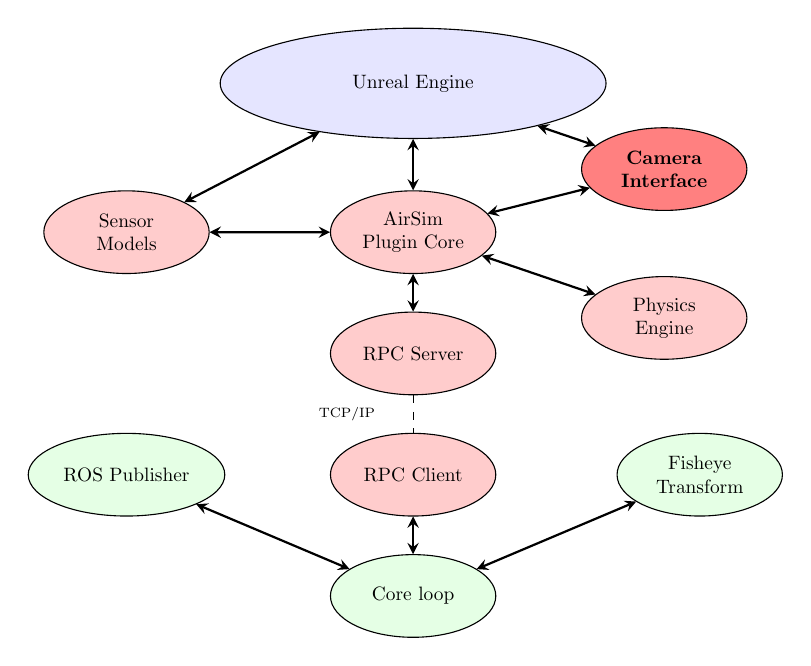
\begin{tikzpicture}[node distance=2.2cm, transform shape, scale=0.7]
        \tikzstyle{topblob} = [ellipse, minimum width = 7cm, minimum height = 2cm, text centered, draw=black, fill=blue!10]
        \tikzstyle{blob} = [ellipse, minimum width = 3cm, minimum height = 1.5cm, text centered, draw=black, fill=red!20]
        \tikzstyle{emphblob} = [ellipse, minimum width = 3cm, minimum height = 1.5cm, text centered, draw=black, fill=red!50]
        \tikzstyle{ownblob} = [ellipse, minimum width = 3cm, minimum height = 1.5cm, text centered, draw=black, fill=green!10]
        \tikzstyle{doublearrow} = [thick, <->, >=stealth]
        \tikzstyle{tcp} = [dashed]
        
        \node (UE) [topblob]{Unreal Engine};
        \node (AirSim) [blob, below of=UE, align=center, yshift=-0.5cm]{AirSim \\ Plugin Core};
        \node (Sens) [blob, left of=AirSim, align=center, xshift=-3cm]{Sensor \\ Models};
        \node (Phys) [blob, below right of=AirSim, align=center, xshift=3cm]{Physics \\ Engine};
        \node (cam) [emphblob, above of=Phys, align=center, yshift=0.5cm]{\textbf{Camera} \\ \textbf{Interface}};
        \node (RPCS) [blob, below of=AirSim]{RPC Server};
        \node (RPCC) [blob, below of=RPCS]{RPC Client};
        \node (Client) [ownblob, below of=RPCC]{Core loop};
        \node (Fish) [ownblob, right of=RPCC, xshift=3cm, align=center]{Fisheye \\ Transform};
        \node (ROS) [ownblob, left of=RPCC, xshift=-3cm, align=center]{ROS Publisher};
        
        \draw[doublearrow] (UE) -- (AirSim);
        \draw[doublearrow] (UE) -- (Sens);
        \draw[doublearrow] (UE) -- (cam);
        \draw[doublearrow] (AirSim) -- (Phys);
        \draw[doublearrow] (AirSim) -- (cam);
        \draw[doublearrow] (AirSim) -- (Sens);
        \draw[doublearrow] (AirSim) -- (RPCS);
        \draw[tcp] (RPCS) -- (RPCC); \node (tcpText) [left of=RPCC, , xshift=1cm, yshift=1.1cm]{\scriptsize TCP/IP};
        \draw[doublearrow] (RPCC) -- (Client);
        \draw[doublearrow] (Client) -- (Fish);
        \draw[doublearrow] (Client) -- (ROS);
        
    \end{tikzpicture}
    \caption{Simplified code interaction within the simulator. Red nodes belong to the AirSim plugin, while Green nodes are custom made for this project. The emphasized node represent modified AirSim code.}
    \label{fig:comm_pattern}
\end{figure}

The project will be implemented for the multirotor game mode. This means that it will not run on the other game modes. The reason for this is that the cameras need to be set up specifically for each game mode, through the Unreal Engine Blueprints imported by the game mode. The fisheye camera and ROS interface will depend on the C++ RPC client API, the perspective camera model and the image capture module for AirSim. The contribution of the project will be to combine perspective images into a single fisheye lens-distorted image, with as few changes as possible to the AirSim plugin. In addition to this, it will build upon the C++ API to allow for publishing images to ROS, through the normal ROS publisher interface. Figure~\ref{fig:comm_pattern} shows the main communication flow of Unreal Engine, AirSim, and the fisheye camera. As the project does not involve HITL with PX4, Mavlink or any controller setup, they are not shown in the figure, and will not be discussed any further in this report.

\section{Implementation}

The goal of the implementation is to get a fisheye camera working and to publish the images to ROS. As only perspective cameras are available, and the fact that they are mounted to specific parts of the multirotor, it was not possible to implement this without making changes to AirSim. However, it was decided early on that no changes would be made to the source code of Unreal Engine. While some changes had to be made to the API in order to implement the ROS node, all of the old API is still functioning and usable.

While most of this report describes angles in degrees, all of the implementations are done using radians. This decision was made to ensure correct scaling when calculating distortion, as well as for consistency in order to reduce human errors.

\subsection{Early development} \label{sec:Early_dev}

As described in Section~\ref{sec:simulator_related}, Unreal Engine supports capturing of cube maps, which is a technique capturing the whole scene through rendering six $90^\circ$ FoV pictures. These are then stored in a special structure, with tooling for projecting it onto a sphere or to a plane using equireclinear projection. As the texture mapping tool for cube maps incorporate radial distortion, it was a natural starting point for simulating fisheye lenses. It is also used in \cite{UnrealCubeCapture}, where they describe using it in their omnidirectional video for their game.

There are various tutorials of how to capture $360^\circ$ screenshots, and many of them are using the Nvidia Ansel plugin \cite{SceenshotsAnsel}. While this made omnidirectional images of the scene, there was no way of processing the images directly, except by saving them locally and loading the images through OpenCV or by similar means. While this is definitely possible, it would create unnecessary save and load cycles. In addition to this, the performance of saving and loading images from disk varies heavily from computer to computer.

\begin{figure}[!htb]
    \centering
    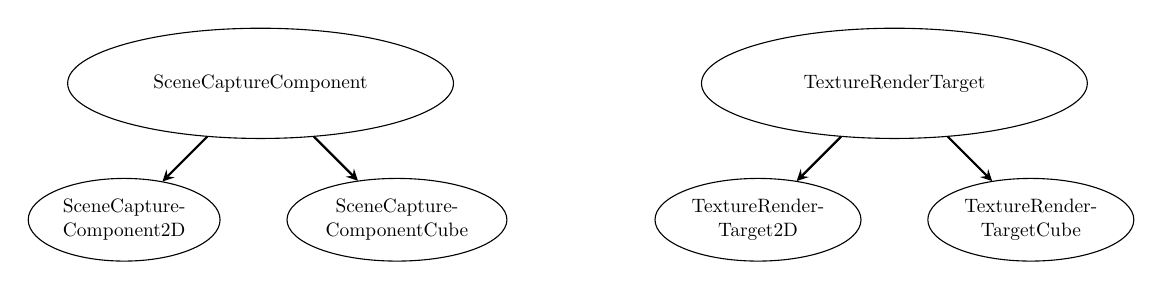
\begin{tikzpicture}[node distance=3.5cm, transform shape, scale=0.7]
        \tikzstyle{topblob} = [ellipse, minimum width = 7cm, minimum height = 2cm, text centered, draw=black]
        \tikzstyle{blob} = [ellipse, minimum width = 3cm, minimum height = 1.5cm, text centered, draw=black]
        \tikzstyle{singlearrow} = [thick, ->, >=stealth]
        
        \node (cap) [topblob]{SceneCaptureComponent};
        \node (cap2d) [blob, below left of=cap, align=center]{SceneCapture- \\ Component2D};
        \node (cap3d) [blob, below right of=cap, align=center]{SceneCapture- \\ ComponentCube};
        \draw[singlearrow] (cap) -- (cap2d);
        \draw[singlearrow] (cap) -- (cap3d);
        
        \node (rend) [topblob, right of=cap, xshift=8cm]{TextureRenderTarget};
        \node (rend2d) [blob, below left of=rend, align=center]{TextureRender- \\ Target2D};
        \node (rend3d) [blob, below right of=rend, align=center]{TextureRender- \\ TargetCube};
        \draw[singlearrow] (rend) -- (rend2d);
        \draw[singlearrow] (rend) -- (rend3d);
        
    \end{tikzpicture}
    \caption{Unreal Engine Capture Component and Render Target class inheritance.}
    \label{fig:capture_render_inherit}
\end{figure}

The second approach involved modifying the capture request and processing system in AirSim directly, to allow requests of both perspective images and cube maps through the existing API. Each camera actor in Unreal Engine needs a capture component and a render target in order to know what to capture and where to store the data. In AirSim's camera setup and API, only the 2D version shown in Figure~\ref{fig:capture_render_inherit} is implemented. Adding support for cube captures would therefore either mean to write alternative cube capture versions of most of the modules shown in Figure~\ref{fig:comm_pattern_camera_request}, or handle both through types through pointers to their parent class.
 
Figure~\ref{fig:comm_pattern_camera_request} shows a simplified data flow in an image request for a perspective image. The arrows represent header file inclusions, where low opacity refers to function calls during setup and dashed arrows represent structure includes. The modules are simplified and many of them encapsulate multiple source code files.

\begin{figure}[!htb]
    \centering
    \tikzstyle{topblob} = [ellipse, minimum width = 7cm, minimum height = 2cm, text centered, draw=black, fill=blue!10]
    \tikzstyle{blob} = [ellipse, minimum width = 3cm, minimum height = 1.5cm, text centered, draw=black, fill=red!10]
    \tikzstyle{structs} = [rectangle, rounded corners, minimum width = 3cm, minimum height = 2cm, text centered, draw=black, fill=red!10]
    \tikzstyle{singlearrow} = [thick, ->, >=stealth]
    \tikzstyle{doublearrow} = [thick, <->, >=stealth]
    \tikzstyle{dashedarrow} = [thick, dashed, ->, >=stealth]
    \tikzstyle{tcp} = [dashed]
    
    \newcommand{\drawdashedarrow}{\raisebox{2pt}
    {\tikz{\draw[dashedarrow](0mm,0mm)--(4.25mm,0mm);}}}
    \newcommand{\drawarrow}{\raisebox{2pt}
    {\tikz{
        \draw[singlearrow](0mm,0mm)--(4.25mm,0mm);
        \draw[doublearrow](5mm,0mm)--(9.25mm,0mm);}}}
    \newcommand{\drawopacitydarrow}{\raisebox{2pt}
    {\tikz{
        \draw[singlearrow, opacity=0.5](0mm,0mm)--(4.25mm,0mm);
        \draw[doublearrow, opacity=0.5](5mm,0mm)--(9.25mm,0mm);}}}
    
    \begin{tikzpicture}[node distance=2.2cm, transform shape, scale=0.7]

        \node (UE) [topblob]{Unreal Engine};
        \node (PIP) [blob, below of=UE, align=center, yshift=-0.5cm]{Perspective \\ Camera};
        \node (setup) [blob, left of=PIP, align=center, xshift=-2cm]{Multirotor \\ Setup};
        \node (Render) [blob, right of=PIP, align=center, xshift=2cm]{Render \\ Request};
        \node (Conv) [blob, right of=Render, align=center, xshift=-0.5cm, yshift=2cm]{Image \\ Convertion};
        \node (UEIMC) [blob, below of=Render, align=center]{Unreal \\ ImageCapture};
        \node (API) [blob, below of=PIP]{Local API};
        \node (RPCS) [blob, below of=API]{RPC Server};
        \node (RPCC) [blob, below of=RPCS]{RPC Client};
        \node (Client) [blob, below of=RPCC]{Client API};
        \node (Struct) [structs, right of=RPCC, align=center, xshift=2cm, yshift=1.1cm]{ImageRequest/ \\ ImageResponse \\ structures};
        
        \draw[doublearrow] (UE) -- (PIP);
        \draw[doublearrow, opacity=0.5] (UE) -- (setup);
        \draw[singlearrow, opacity = 0.5] (PIP) -- (setup);
        \draw[singlearrow] (PIP) -- (UEIMC);
        \draw[singlearrow] (UE) -- (Render);
        \draw[singlearrow] (Conv) -- (Render);
        \draw[singlearrow] (Render) -- (UEIMC);
        \draw[singlearrow] (UEIMC) -- (API);
        \draw[singlearrow] (RPCS) -- (API);
        \draw[singlearrow, opacity=0.5] (setup) -- (API);
        \draw[tcp] (RPCS) -- (RPCC); \node (tcpText) [left of=RPCC, , xshift=1cm, yshift=1.1cm]{\scriptsize TCP/IP};
        \draw[singlearrow] (RPCC) -- (Client);
        \draw[dashedarrow] (Struct) -- (UEIMC);
        \draw[dashedarrow] (Struct) -- (API);
        \draw[dashedarrow] (Struct) -- (Client);
        
    \end{tikzpicture}
    \caption{Simplified overview of dependencies in an AirSim image request. Dashed arrows (\protect\drawdashedarrow) represent structure includes and whole arrows (\protect\drawarrow)represent function includes, low opacity arrows (\protect\drawopacitydarrow) represent dependencies during setup.}
    \label{fig:comm_pattern_camera_request}
\end{figure}

As writing alternative modules for AirSim to handle cube captures was deemed to be too large a task, the second option was chosen. Although this meant that more of the code was reusable, it quickly got out of hand. Since the respective child classes carry much of the implementation details for the capture modes, a lot of casting back and forth between types had to be implemented. This not only created code which was hard to read, but it also meant that much less of the original code was reusable than originally thought. Inexperience with advanced object-oriented C++ also created a huge time sink, using more time on fixing type-casting related problems than actual implementation.

\subsection{Final implementation overview} \label{subsec:Fisheye_impl_overview}

The final version of the fisheye camera is implemented as a client-side program, meaning that it is separated from both the AirSim plugin and Unreal Engine. This means that features of Unreal Engine that are not available through the AirSim API will no longer be available to the fisheye camera. As cube maps no longer are available, the fisheye image will have to be made by manually combining perspective images. Since there are no fisheye cameras with a vertical FoV greater than $270^\circ$, and the fact that the camera is mounted beneath the multirotor, the camera was implemented using a setup of 5 perspective cameras with a FoV of $90^\circ$. This can be extended to a full cube map, providing $360^\circ$ vertical FoV, by adding one extra camera to the multirotor model in Unreal Engine. The aspect ratio $\rho$ was also set to be $1$, matching that of normal cube maps. 
In order to be able to get the correct images, the camera setup on the multirotor model had to be changed. As seen in Figure~\ref{fig:new_Blueprint_multirotor}, the 5 cameras are clustered below the multirotor at a $90^\circ$ offset from one another, with the main direction being downwards. As the number of cameras and their name reference is hardcoded into AirSim, some changes had to be made to the camera interface. This consisted of adding references to the new cameras for the link between AirSim and Unreal Engine and new API entries for the AirSim camera API.

\begin{figure}[!htb]
    \centering
    \begin{subfigure}{0.45\linewidth}
        \centering
        \includegraphics[height=4cm]{rapport/fig/Simulator/camera_setup.png}
        \caption{Fisheye camera setup}
        \label{fig:new_Blueprint_cameras}
    \end{subfigure}
    \begin{subfigure}{0.45\linewidth}
        \centering
        \includegraphics[height=4cm]{rapport/fig/Simulator/camera_setting.png}
        \caption{Downward camera settings}
        \label{fig:new_Blueprint_nodes}
    \end{subfigure}
    \caption{Multirotor Blueprint setup for the fisheye camera, consisting of 5 clustered perspective cameras.}
    \label{fig:new_Blueprint_multirotor}
\end{figure}

The following sections will present the modeling of the fisheye camera. The steps described are done on a pixel-wise level. As the same operation is done to every pixel in the source images, without any dependencies between them, this a highly parallelizable task, making it ideal for GPU acceleration.

\subsection{Combining pictures} \label{sec:combining_pictures}

The response form AirSim when requesting an image is an image response structure containing; camera name, position, orientation, time stamp, image dimensions, the image type, and the image data. It also contains whether the image has been compressed to a PNG format. This field is however irrelevant as the fisheye camera will request raw RGBA8 pictures in order to do the mapping.

\begin{figure}[!htb]
    \centering
    \tdplotsetmaincoords{70}{160}
    \begin{tikzpicture}[tdplot_main_coords, scale = 1.4]
    
    \coordinate (O) at (0,0,0);
    \tdplotsetrotatedcoords{0}{-90}{90}
    
    \coordinate (IMBOTC) at (0,0,-2);
    \tdplotsetrotatedcoordsorigin{(IMBOTC)}
    \draw[tdplot_rotated_coords, thick, fill=black!8, opacity=1.0] (2,0,2) -- (2,0,-2) -- (-2,0,-2) -- (-2,0,2) -- cycle;
    
    \coordinate (IMLEFT) at (0,-2,0);
    \tdplotsetrotatedcoordsorigin{(IMLEFT)}
    \draw[tdplot_rotated_coords, thick, fill=black!8, opacity=1.0] (0,2,2) -- (0,-2,2) -- (0,-2,-2) -- (0,2,-2) -- cycle;
    
    
    \tdplotsetrotatedcoordsorigin{(O)}
    
    \draw[tdplot_rotated_coords, ->] (0,0,2) -- (0,0,3) node[below]{$Z$};
    
    \tdplotsetcoord{IMGC}{2}{-90}{0}
    \tdplotsetrotatedcoordsorigin{(IMGC)}
    \draw[thick, tdplot_rotated_coords, fill=black!4, opacity=0.8] (-2,-2,0) -- (-2,2,0) -- (2,2,0) -- (2,-2,0) -- cycle;
    
    \draw[tdplot_rotated_coords, dashed] (0,0,-1.5) -- (0,0,0);
    
    \draw[tdplot_rotated_coords, dashed, opacity=0.8] (0,0,-2) -- (0,-2,0);
    \draw[tdplot_rotated_coords, dashed, opacity=0.8] (0,0,-2) -- (2,0,0);
    \draw[tdplot_rotated_coords, dashed, opacity=0.8] (0,0,-2) -- (2,2,0);
    \draw[tdplot_rotated_coords, dashed, opacity=0.8] (0,0,-2) -- (2,-2,0);
    \draw[tdplot_rotated_coords, dashed, opacity=0.8] (0,0,-2) -- (-2,-2,0);
    
    \tdplotsetrotatedcoordsorigin{(O)}
    \tdplotsetrotatedcoords{90}{70}{0}
    \draw[tdplot_rotated_coords, thick, fill=black!5, opacity = 0.8] (0:2) arc (0:180:2);
    \tdplotsetrotatedcoords{0}{-90}{90}
    \draw[thick, tdplot_rotated_coords, fill=black!3] (0:2) arc (0:360:2);
    
    \tdplotsetrotatedcoords{0}{-90}{90}
    \draw[tdplot_rotated_coords, ->] (-0.5,0,0) -- (3,0,0) node[below]{$X$};
    \draw[tdplot_rotated_coords, ->] (0,-0.5,0) -- (0,2.5,0) node[right]{$Y$};
    \draw[tdplot_rotated_coords, dashed] (0,0,0) -- (0,0,0.6);
    
    \draw[tdplot_rotated_coords, dashed, opacity=0.8] (1.155,1.155,1.155) -- (2,2,2);
    \draw[tdplot_rotated_coords, dashed, opacity=0.8] (1.155,0,1.155) -- (2,0,2);
    \draw[tdplot_rotated_coords, dashed, opacity=0.8] (1.155,-1.155,1.155) -- (2,-2,2);
    
    \draw[tdplot_rotated_coords, dashed, opacity=0.8] (0,0,0) -- (0.5,0.5,0.5);
    \draw[tdplot_rotated_coords, dashed, opacity=0.8] (0,0,0) -- (0.5,0,0.5);
    \draw[tdplot_rotated_coords, dashed, opacity=0.8] (0,0,0) -- (0.5,-0.5,0.5);
    \draw[tdplot_rotated_coords, dashed, opacity=0.8] (0,0,0) -- (0,-0.6,0.6);
    \draw[tdplot_rotated_coords, dashed, opacity=0.8] (0,0,0) -- (-0.7,-0.7,0.7);
    
    
    \tdplotsetcoord{IMTOPC}{2}{0}{-90}
    \tdplotsetrotatedcoordsorigin{(IMTOPC)}
    \draw[tdplot_rotated_coords, thick, fill=black!2, opacity=0.7] (2,0,2) -- (2,0,-2) -- (-2,0,-2) -- (-2,0,2) -- cycle;
    
    \coordinate (IMRIGHT) at (0,2,0);
    \tdplotsetrotatedcoordsorigin{(IMRIGHT)}
    \draw[tdplot_rotated_coords, thick, fill=black!2, opacity=0.7] (0,2,2) -- (0,-2,2) -- (0,-2,-2) -- (0,2,-2) -- cycle;
    
    \end{tikzpicture}
    
    \caption{Projection from perspective camera to a unit sphere using 5 perspective cameras, given a FoV of $180^\circ$.}
    \label{fig:impl_Sphere_projection}
\end{figure}

Figure~\ref{fig:impl_Sphere_projection} shows the setup for the custom cube capture used by the fisheye camera, where each plane represents an image taken by a camera on the multirotor. To provide a correct projection, the angles $\phi$ and $\theta$, shown in Figure~\ref{fig:fisheye_spherical_projection} must be known. In order to convert the pixel positions to these angles, it is beneficial to change to image coordinates on a plane with $x^i,y^i \in [-1,1]$. Here $[x^i, y^i]^\top$ and $[u^i,v^i]^\top$ refer to the image and pixel coordinates on the image plane represented, with the origin in each camera's own coordinate frame. Table~\ref{tab:impl_quaternion_rotations} shows the respective superscripts used to describe each camera frame. Using Equation~\eqref{eq:pixel_transform}, with each camera having an aspect ratio $\rho = 1$, the transformation shown in Equation~\eqref{eq:impl_pixel_inverse_transform} is obtained.

\begin{equation}
    \mathbf{p}^i = \begin{bmatrix}
        x^i \\ y^i \\ 1
    \end{bmatrix} = \begin{bmatrix}
        \frac{W}{2} & 0 & \frac{W}{2} \\
        0 & \frac{H}{2} & \frac{H}{2} \\
        0 & 0 & 1
    \end{bmatrix}^{-1}\begin{bmatrix}
        u^i \\ v^i \\ 1
    \end{bmatrix} = \begin{bmatrix}
        \frac{2}{W} & 0 & -1 \\
        0 & \frac{2}{H} & -1 \\
        0 & 0 & 1
    \end{bmatrix}\begin{bmatrix}
        u^i \\ v^i \\ 1
    \end{bmatrix}
    \label{eq:impl_pixel_inverse_transform}
\end{equation}

A coordinate frame $\bullet^c$ is defined for the fisheye $360^\circ$ camera to be aligned with the coordinate frame of the downward pointing camera. Hence all points $\mathbf{p}^i = [x^i,y^i,z^i]^\top$, where $i$ refers to the superscript assigned to each camera frame, should be rotated to the camera frame. This rotation is shown in Equation~\eqref{eq:impl_rotation}. $\mathbf{R}^d_i$ represents the rotation from fra $i$ to $d$, where $\mathbf{q}_{d,i}$ in Equation~\eqref{eq:impl_rotation_q} represent the same rotation on quaternion form.

\begin{subequations}
    \begin{align}
        \mathbf{p}^c &= \!\begin{aligned}[t]
            \mathbf{p}^d = \begin{bmatrix} x^d \\ y^d \\ z^d \end{bmatrix} &= \mathbf{R}^d_i \mathbf{p}^i
        \end{aligned} \label{eq:impl_rotation_R} \\[0.75ex]
        \mathbf{q}^c &= \!\begin{aligned}[t]
            \mathbf{q}^d = \begin{bmatrix} 0 \\ \mathbf{p}^d \end{bmatrix} &= (\mathbf{q}_{d,i})\mathbf{q}^i(\mathbf{q}_{d,i})^\top
        \end{aligned} \label{eq:impl_rotation_q}
    \end{align}
    \label{eq:impl_rotation}
\end{subequations}

The quaternion rotation in Equation~\eqref{eq:impl_rotation_q} will be implemented in this project. Table~\ref{tab:impl_quaternion_rotations} lists each camera, their defined coordinate frame, as well as the rotation needed for the representative image coordinate vector. $\hat{\theta}$ and $\hat{\phi}$ represent the rotation angle around the local $x-$ and $y-$axis respectively.

\begin{table}[!htb]
    \centering
    \caption{Rotation needed to rotate image coordinate $p^i$ to $p^d$.}
    \label{tab:impl_quaternion_rotations}
    \begin{tabular}{|c|c|c|c|} \hline
        \multirow{2}{*}{Camera Direction} & \multirow{2}{*}{ $\mathbf{p}^i$} & \multirow{2}{*}{$\mathbf{R}^d_i = \mathbf{R}_{x,\hat{\theta}}(\hat{\theta})\mathbf{R}_{y,\hat{\phi}}(\hat{\phi})$} & \multirow{2}{*}{Quaternion $\mathbf{q}_{d,i}$} \\ &&& \\ \hline \hline
        \multirow{2}{*}{Down} & \multirow{2}{*}{$\mathbf{p}^d$} & \multirow{2}{*}{$\hat{\theta} = 0$, $\hat{\phi} = 0$} & \multirow{2}{*}{$[1,0,0,0]^\top$} \\ &&& \\ \hline
        \multirow{2}{*}{Front} & \multirow{2}{*}{$\mathbf{p}^f$} & \multirow{2}{*}{$\hat{\theta} = \frac{\pi}{2}$, $\hat{\phi} = 0$} & \multirow{2}{*}{$\left[\frac{\sqrt{2}}{2},\frac{\sqrt{2}}{2},0,0\right]^\top$} \\ &&& \\ \hline
        \multirow{2}{*}{Right} & \multirow{2}{*}{$\mathbf{p}^r$} & \multirow{2}{*}{$\hat{\theta} = \frac{\pi}{2}$, $\hat{\phi} = \frac{\pi}{2}$} & \multirow{2}{*}{$[0.5,0.5,0.5,0.5]^\top$} \\ &&& \\ \hline
        \multirow{2}{*}{Back} & \multirow{2}{*}{$\mathbf{p}^b$} & \multirow{2}{*}{$\hat{\theta} = \frac{\pi}{2}$, $\hat{\phi} = \pi$} & \multirow{2}{*}{$\left[0,0,\frac{\sqrt{2}}{2},\frac{\sqrt{2}}{2}\right]^\top$} \\ &&& \\ \hline
        \multirow{2}{*}{Left} & \multirow{2}{*}{$\mathbf{p}^l$} & \multirow{2}{*}{$\hat{\theta} = \frac{\pi}{2}$, $\hat{\phi} = -\frac{\pi}{2}$} & \multirow{2}{*}{$\left[0.5,0.5,-0.5,-0.5\right]^\top$} \\ &&& \\ \hline
    \end{tabular}
\end{table}

After rotating the image coordinate to the camera frame, the feature unit vector $[\theta, \phi]^\top$ can be calculated using Equation~\eqref{eq:theory_polar_coords}. This calculation is shown in Equation~\eqref{eq:impl_polar_transform}. The arc tangent is implemented using the standard library \emph{atan2(y,x)}-function. This provides extra functionality for calculating the quadrant of the angle. The result is therefore in the range $[-\pi,\pi]$, which is needed for correct picture placement.

\begin{subequations}
    \begin{equation}
        \theta = atan2\left(y^c,x^c\right)
        \label{eq:impl_polar_transform_theta}
    \end{equation}
    \begin{equation}
        \phi = atan2\left(\sqrt{(x^c)^2 + (y^c)^2},z^c\right)
        \label{eq:impl_polar_transform_phi}
    \end{equation}
    \label{eq:impl_polar_transform}
\end{subequations}

\subsection{Lens implementation} \label{sec:lens_modeling}

The camera lens is implemented with the polynomial model presented in Table~11.1 in \cite{FisheyeCorke}. For now this is implemented as the fourth order polynomial in Equation~\eqref{eq:impl_lens_model}, where the parameters $k_1$-$k_4$ are tunable distortion parameters. $r(\phi)$ and $\theta$ refer to the polar coordinates of the fisheye image plane, defining the feature position in the fisheye image.

\begin{align}
    \begin{aligned}[t]
    r(\phi) &= k_1 \phi + k_2 \phi^2 + k_3 \phi^3 + k_4 \phi^4 \\[0.75ex]
    \theta &= \theta
    \end{aligned}
    \label{eq:impl_lens_model}
\end{align}

The polynomial model is flexible and easy to implement, while able to simulate most effects caused by radial distortion. Unfortunately, as the model does not have any dependency on the longitude $\theta$, it is not able to simulate the effects of tangential distortion and this will have to be implemented in the future.

In order to produce the final picture, the polar coordinates have to be transformed back to pixel coordinates for the new image. Again using $W$ as the width and $H$ as the height in pixels, the transformation can be found using Equation~\eqref{eq:pixel_transform}, as well as the relationship between polar and Cartesian coordinates shown in Equation~\eqref{eq:theory_equiangular_coords}. The resulting transformation is shown in Equation~\eqref{eq:impl_pixel_transform_final}.

\begin{equation}
    \begin{bmatrix}
        u \\ v \\ 1
    \end{bmatrix} = \begin{bmatrix}
        \frac{W}{2x_{max}} & 0 & \frac{W}{2} \\
        0 & \frac{H}{2y_{max}} & \frac{H}{2} \\
        0 & 0 & 1
    \end{bmatrix}\begin{bmatrix}
        x \\ y \\ 1
    \end{bmatrix} =
    \begin{bmatrix}
        \frac{W}{2x_{max}} & 0 & \frac{W}{2} \\
        0 & \frac{H}{2y_{max}} & \frac{H}{2} \\
        0 & 0 & 1
    \end{bmatrix}\begin{bmatrix}
        r(\phi) cos(\theta) \\ r(\phi) sin(\theta) \\ 1
    \end{bmatrix}
    \label{eq:impl_pixel_transform_final}
\end{equation}

Assuming the the fisheye image will the whole square image, $y_{max} = x_{max}$ can be calculated to be calculated as shown in Equation~\eqref{eq:impl_size_xy_max}, with $\phi_{max}=\frac{\Theta}{2}=\frac{3 \pi}{2}$.

\begin{equation}
    \begin{aligned}
        x_{max} = y_{max} &= ||k_1 \phi_{max} + k_2 \phi_{max}^2 + k_3 \phi_{max}^3 + k_4 \phi_{max}^4 ||_2 \\
        &= \left|\left| \left(\frac{3 \pi}{4}\right)k_1 + \left(\frac{3 \pi}{4}\right)^2 k_2 + \left(\frac{3 \pi}{4}\right)^3 k_3 + \left(\frac{3 \pi}{4}\right)^4 k_4 \right|\right|_2
    \end{aligned}
    \label{eq:impl_size_xy_max}
\end{equation}

If this is not the case, meaning that there is a mismatch between the size of the image plane and the size of the photosensitive element of the camera, then $x_{max}$ and $y_{max}$ needs to be calculated based on the pixel dimensions of the image sensor. This calculation is shown in Equation~\eqref{eq:impl_size_xy_max_nomatch}, where $w$ is the pixel width and $h$ is the pixel height.

\begin{equation}
    \begin{aligned}
        x_{max} &= w\frac{W}{2} \\
        y_{max} &= h \frac{H}{2}
    \end{aligned}
    \label{eq:impl_size_xy_max_nomatch}
\end{equation}


% \subsection{Code structure}

% The fisheye module is made to be included as a library into other projects, along with it's header file. The module defines a FisheyeTransformer class and the Lens, SourceImage and TeansformRequest structures. SourceImage contains the one perspective 

% \begin{figure}
%     \centering
%     \begin{tikzpicture}[node distance = 4cm, transform shape, scale=1.0]
%         \tikzstyle{class} = [rectangle, minimum width=3cm, minimum height = 3cm, text centered, draw=black, fill=blue!10]
%         \tikzstyle{struct} = [rectangle, minimum width=3cm, minimum height = 3cm, text centered, draw=black, fill=green!10]
        
%         \node (FET) [class, align=center, rectangle split, rectangle split parts=2]{
%             \textbf{FisheyeTransformer}
%             \nodepart{second} \begin{flushleft}+\end{flushleft} test
%         };
        
%     \end{tikzpicture}
%     \caption{Caption}
%     \label{fig:my_label}
% \end{figure} Add this?

\subsection{ROS interface to AirSim and fisheye camera}\label{subsec:ROS_interface}

The ROS node implementation is split into two different parts. The first part handles the core loop of the program, sending AirSim ImageRequests and handling the fisheye transformations, while the other handles ROS publishing. To be able to do this the ROS package inherits the base RPC-Client API class defined for AirSim, along with including the ROS header, to create a link between the two. However, for the added functionality of publishing fisheye images, it also depends on the fisheye module, OpenCV and cv\_bridge\footnote{https://github.com/ros-perception/vision\_opencv}, where cv\_bridge handles the conversion between the OpenCV image object and the ROS image message.

\begin{figure}[!htb]
    \centering
    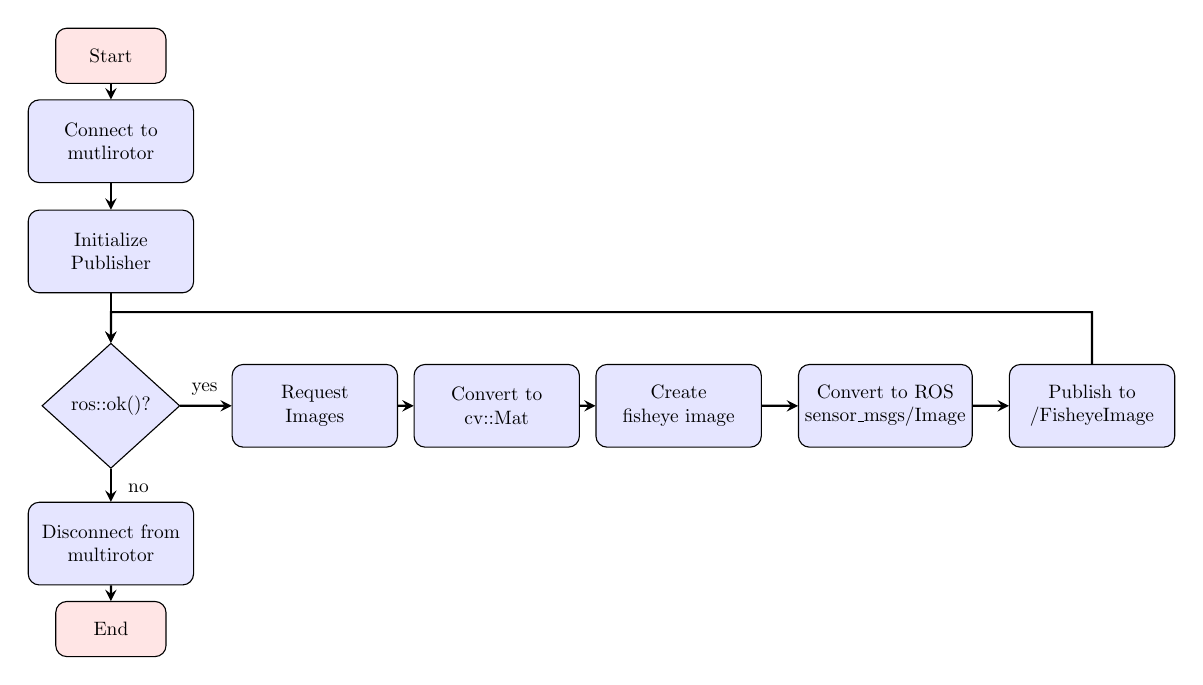
\begin{tikzpicture}[node distance=2cm, transform shape, scale=0.7]
        \tikzstyle{start} = [rectangle, rounded corners, minimum width = 2cm, minimum height = 1cm, text centered, draw=black, fill=red!10]
        \tikzstyle{if} = [diamond, minimum width = 2.5cm, minimum height = 1.5cm, text centered, draw=black, fill=blue!10]
        \tikzstyle{task} = [rectangle, rounded corners, minimum width = 3cm, minimum height = 1.5cm, text centered, draw=black, fill=blue!10]
        \tikzstyle{singlearrow} = [thick, ->, >=stealth]
        
        \node (START) [start]{Start};
        \node (CONN) [task, below of=START, align=center, yshift=0.45cm]{Connect to \\ mutlirotor};
        \node (PUBINIT) [task, below of=CONN, align=center]{Initialize \\ Publisher};
        
        \node (ROSOK) [if, below of=PUBINIT, yshift=-0.8cm]{ros::ok()?};
        \draw[] (ROSOK) node[xshift=1.7cm, yshift=0.3cm]{yes};
        \draw[] (ROSOK) node[xshift=0.5cm, yshift=-1.5cm]{no};
        \node (REQ) [task, align=center, right of=ROSOK, xshift=1.7cm]{Request \\ Images};
        \node (OPENCV) [task, align=center, right of=REQ, xshift=1.3cm]{Convert to \\ cv::Mat};
        \node (FISH) [task, align=center, right of=OPENCV, xshift=1.3cm]{Create \\ fisheye image};
        \node (CONV) [task, align=center, right of=FISH, xshift=1.75cm]{Convert to ROS \\ sensor\_msgs/Image};
        \node (PUB) [task, align=center, right of=CONV, xshift=1.75cm]{Publish to \\ /FisheyeImage};
        
        \node (DISC) [task, align=center, below of=ROSOK, yshift=-0.5cm]{Disconnect from \\ multirotor};
        \node (END) [start, below of=DISC, yshift=0.45cm]{End};
        
        \draw[singlearrow] (START) -- (CONN);
        \draw[singlearrow] (CONN) -- (PUBINIT);
        \draw[singlearrow] (PUBINIT) -- (ROSOK);
        \draw[singlearrow] (ROSOK) -- (REQ);
        \draw[singlearrow] (REQ) -- (OPENCV);
        \draw[singlearrow] (OPENCV) -- (FISH);
        \draw[singlearrow] (FISH) -- (CONV);
        \draw[singlearrow] (CONV) -- (PUB);
        \path[draw, -latex, singlearrow] (PUB) -- ++(0cm,1.7cm) -| (ROSOK);
        \draw[singlearrow] (ROSOK) -- (DISC);
        \draw[singlearrow] (DISC) -- (END);
        
    \end{tikzpicture}
    \caption{ROS publisher loop.}
    \label{fig:impl_ROS_pub_loop}
\end{figure}

Using the custom setup discussed in Section~\ref{subsec:Fisheye_impl_overview}, the requests for the perspective images are treated by referencing the cameras by name, as there is no way of polling AirSim to get the available cameras. The received vector of images is then converted to OpenCV images and wrapped into a custom FisheyeImageRequest made for this project. This structure holds the images, image size, and information about the camera pose, which is necessary to compute the final image.

The created ROS node runs an infinite loop, shown in Figure~\ref{fig:impl_ROS_pub_loop} and it is interruptable by crtl+c through the ros::ok() function. The loop consists of polling for images, transformation to fisheye-image, and publishing the image on the FisheyImage ROS topic. In order to control the multirotor, the old client API needs to be included and used in the core loop of the client application. Both the ROS publisher and the old client API can run simultaneously.


\cleardoublepage

\chapter{Results and Discussion}

\section{performance}

\subsection{compile time and runtime calculations}

\subsection{optimization}

\subsection{Discussion}
% This decision was made in order to separate the implementation into its own module, and thereby reducing the impact of changes to AirSim. As AirSim is still developed heavilly upon, it was seen as a way to reduce the amount trouble induced by changes to the core code of the plugin. This would also allow me to more often integrate the bug fixes and new implementations they made, without ruining my ownw work. The downside of this decision is that it removes possibility to use any features in Unreal Engine which is not implemented in the AirSim API. 
\cleardoublepage
%===================================== CHAP 5 =================================

\chapter{Conclusion and further work}

\cleardoublepage

%% PART 4
\input{references.tex}	%% Edit your references in "mylib.bib"
%\input{appendix.tex}

\end{document}